\documentclass[9pt,shortpaper,twoside,web]{ieeecolor2}
\usepackage{generic}
\usepackage{cite}
\usepackage{amsmath,amssymb,amsfonts}
\usepackage{graphicx}
\usepackage{textcomp}
\usepackage{booktabs}
\usepackage{multirow}
\usepackage{array}
\usepackage{algorithm}
\usepackage{algpseudocode}
\usepackage{xcolor}
\usepackage{url}

% --- editing macros: remove before submission -------------------------
\newcommand{\tbd}[1]{\textcolor{red}{[TODO: #1]}}
\newcommand{\NUMQ}[1]{\textcolor{red}{[NUMBER?: #1]}}
\newcommand{\NQ}{\textcolor{red}{[?]}}
% session names
\newcommand{\Sval}{S-val}
\newcommand{\Stest}{S-test}
\newcommand{\Snew}{S-new}
\newcommand{\Sctrl}{S-ctrl}
% ORB-SLAM3 modes
\newcommand{\fullslam}{\emph{full SLAM}}
\newcommand{\loconly}{\emph{localisation only}}
\newcommand{\reloc}{\emph{each frame relocalised}}

\def\BibTeX{{\rm B\kern-.05em{\sc i\kern-.025em b}\kern-.08em
    T\kern-.1667em\lower.7ex\hbox{E}\kern-.125emX}}
\markboth{\journalname, VOL. XX, NO. XX, XXXX 2023}
{Author \MakeLowercase{\textit{et al.}}: Probe-Mounted RGB-D Tracking by Self-Mapped Scene Coordinate Regression}

\begin{document}
\title{Freehand 3D Ultrasound Without an External Tracker: Probe-Mounted RGB-D Tracking by Self-Mapped Scene Coordinate Regression}

\author{Ruixuan~Li, Yipeng~Hu$^\star$, and Emmanuel~Vander~Poorten%
\thanks{R. Li and E. Vander Poorten are with the Robot-Assisted Surgery group, KU Leuven, Leuven, Belgium (e-mail: ruixuan.li@kuleuven.be).}%
\thanks{Y. Hu is with the Dept of Med Phys \& Biomedical Eng, UCL, London, UK}
\thanks{This project received funding from FWO projects 12A8N26N and V444626N.}}

\maketitle

\begin{abstract}
\textcolor{cyan}{Objective:} Freehand three-dimensional (3D) ultrasound (US) needs the six-degree-of-freedom pose of every US image, usually from an external tracker. We present a data-driven alternative using a probe-mounted RGB-D camera alone, and establish when it suffices for 3D compounding. \textcolor{cyan}{Methods:} The operator first scans the room with the probe camera for 1--2\,min. One scene coordinate regression network maps this scan itself, trains on its own labels, and localises every examination frame independently by a Kabsch RANSAC fit to the measured depth. We evaluated 63 test sweeps (three sessions, one room, two subjects, a phantom) against an optical tracker and compared with ORB-SLAM3. \textcolor{cyan}{Results:} With a room scan along the examination views, the error at the US image was 2.2--3.1\,mm (shape 1.7--1.9\,mm), 0.4--0.5\,mm above the same network trained on tracker poses. A scan missing these views raised the error on the same sweeps from 2.28 to 13.57\,mm (10.95\,mm with tracker labels). With an occluder covering 30--60\,\% of the image width, our error rose by at most 0.9\,mm on average (no sweep above 8.5\,mm), whereas ORB-SLAM3 failed on single sweeps by 13--132\,mm while reporting successful tracking. \textcolor{cyan}{Conclusion:} Per-frame localisation against a self-mapped learned room model is a feasible tracker-free alternative when the room scan covers the examination views; it trades accuracy for a bounded error and detectable failures. \textcolor{cyan}{Significance:} It removes external tracking hardware, and its operating conditions give a scanning protocol with pre-examination checks.
\end{abstract}


\begin{IEEEkeywords}
Freehand 3D ultrasound, probe tracking, scene coordinate regression, RGB-D camera, visual relocalisation.
\end{IEEEkeywords}



\section{Introduction}
\label{sec:introduction}

\IEEEPARstart{F}{reehand} three-dimensional (3D) ultrasound (US) reconstructs a volume from 2D images acquired while the operator sweeps a conventional probe, giving access to organ and lesion volumes, vessel courses and planes for needle guidance \cite{TODO-3dus-clinical-applications}. Reconstruction needs the six-degree-of-freedom (6-DoF) pose of every image, which in practice comes from an optical or electromagnetic tracker \cite{TODO-freehand-3dus-review}. Optical tracking needs a line of sight that the operator, the patient and staff interrupt; electromagnetic tracking needs a field generator next to the patient and is disturbed by metal \cite{TODO-em-tracking-distortion}. Both must be installed and calibrated in each room, which rules them out where a volume would be useful at short notice: at the bedside, in the emergency department, or in a crowded operating room \cite{TODO-point-of-care-3dus}.

A replacement does not have to match optical tracking; it has to be good enough for compounding, which we take as about 2--3\,mm at the US image, of the order of the elevational beam width \cite{TODO-elevational-beamwidth}. For a camera on the probe, rotation dominates this budget: the image lies about 16\,cm from the camera, so $1^\circ$ of rotation moves it by up to 2.8\,mm.

A replacement must also give an absolute pose for every frame, need no preparation of the room or the patient, and keep everything on the probe; existing approaches give up at least one of these. Sensorless methods estimate probe motion from the US images: classically from speckle decorrelation \cite{TODO-speckle-decorrelation}, and with deep networks from consecutive frames \cite{prevost2018}, multi-frame context \cite{guo2023tbme} or longer temporal context \cite{li2024longterm}, compared on a common dataset in the TUS-REC2024 challenge \cite{li2025tusrec}. A coupling pad with N-shaped lines adds a reference visible in the image \cite{dai2024coupling}; without such a reference, these methods integrate relative motion, so the error grows along the sweep, and they must generalise across subjects and protocols. Probe-mounted cameras have mostly been used in the same relative way: Sun et al.\ \cite{sun2014skin} tracked skin features and built a skin map by visual SLAM, so the poses are relative to the skin and errors accumulate with the distance travelled, and visual--inertial odometry needs no prepared scene but drifts \cite{buchanan2024vio,he2024probemounted}. Absolute camera-based methods rely on something prepared in advance: ProbeSight localises a probe camera against a prior high-resolution surface map of the anatomy by inverse rendering \cite{wang2017probesight}; Huang et al.\ \cite{huang2025lightweight} regress the probe pose from two lightweight cameras relative to a workspace with coloured markers; and Zhang et al.\ align camera images with a simulated replica of a textured workspace \cite{zhang2025servoing} and combine global visual guidance with local B-mode cues \cite{zhang2026seeing}. MLRecon tracks the probe from an external RGB-D camera without markers \cite{zhang2026mlrecon}, which brings back a line-of-sight constraint.

RGB-D simultaneous localisation and mapping (SLAM) meets all three requirements. Closest to our set-up, Busam et al.\ \cite{busam2018insideout} mounted an RGB-D camera of the same family on a transrectal probe, facing away from the patient, tracked it by visual SLAM against a map of the operating room, and compared the resulting 3D US compounding with an optical tracker. Keypoint-based systems such as ORB-SLAM3 \cite{campos2021orbslam3} represent the room by keypoints, track them from frame to frame, optimise keyframes by bundle adjustment and relocalise by place recognition when tracking is lost; they are the natural reference for any tracker-free design. Visual relocalisation obtains an absolute pose from a single image instead. Absolute pose regression maps an image directly to a pose \cite{TODO-posenet}, but such networks behave more like image retrieval than geometric estimation, which limits their accuracy \cite{sattler2019}. Scene coordinate regression (SCR) instead predicts dense image-to-scene correspondences and solves the pose robustly. It was introduced with regression forests on RGB-D images \cite{shotton2013}, adapted to new scenes online \cite{cavallari2017onthefly,cavallari2019online}, trained end to end through a differentiable RANSAC in DSAC* \cite{brachmann2022dsac}, made fast to train by ACE \cite{brachmann2023ace}, and improved for viewpoints far from the mapping images by ACE-G \cite{bruns2025aceg}. ACE0 removes the need for mapping poses by alternating between training the relocaliser on the images registered so far and registering further images with it \cite{brachmann2024ace0}, and ACE-SLAM uses SCR as the map of a real-time RGB-D SLAM system, training it online \cite{alzugaray2025aceslam}. In medicine, relocalisation against a prior reconstruction has been studied mainly in endoscopy, where the map is of the anatomy \cite{TODO-endoscopic-relocalisation}; to our knowledge, SCR has not been used for freehand 3D US.

\begin{figure*}[t]
  \centering
  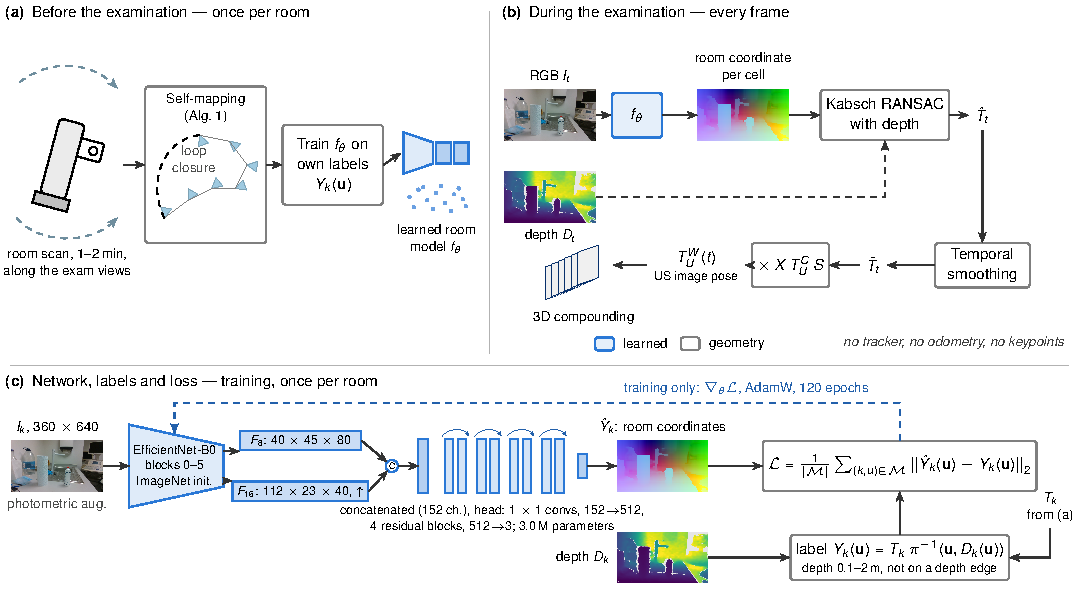
\includegraphics[width=0.90 \linewidth]{fig_overview.pdf} 
  \caption{System overview. (a)~Before the examination, once per room: the operator scans the room for 1--2\,min with the RGB-D camera on the probe, along the examination views; the scene coordinate network maps this room scan itself (Algorithm~\ref{alg:mapping}) and is trained on the resulting labels. (b)~During the examination, for every frame: the network predicts the room coordinate of every image cell from the RGB image, a Kabsch RANSAC fit with the measured depth gives the camera pose, temporal smoothing combines neighbouring poses, and the probe calibration gives the pose of the US image. The network is the only learned component.}
  \label{fig:overview}
\end{figure*}

We take a different, data-driven route: we keep the inside-out set-up of \cite{busam2018insideout} but replace SLAM by per-frame relocalisation against a learned model of the room, built from a 1--2\,min scan with the probe camera before the examination. An SCR network predicts, for every image cell, the 3D room point it observes, and the pose follows from an exact fit to the measured depth. The network only has to memorise one room, and RANSAC over thousands of dense correspondences discards cells on moved objects or hands. The network maps the room scan itself, following the scheme of ACE0, but it uses the measured depth for metric labels, ICP seeding and extension and a 3D--3D solver, refines the poses by a pose graph with ICP loop closures instead of joint refinement, and adds a camera-frame probe calibration, so no tracker is needed to build the map. Unlike ACE-SLAM, we map once before the examination and keep the network fixed. There is no tracking state that can be lost or carry a wrong pose forward, and the accuracy is fixed by the map before the first sweep: the map, and how the room scan is recorded, become the object of study.

We ask four questions on 63 test sweeps in three sessions: what removing the tracker from mapping costs, what decides the accuracy, how a learned per-frame localiser compares with RGB-D SLAM, and when it fails. With a room scan along the examination views, the error at the US image is 2.2--3.1\,mm, 0.4--0.5\,mm more than with tracker labels. A scan that misses these views costs about 9\,mm even with perfect labels, because the network cannot place viewpoints it has not seen. ORB-SLAM3 is more accurate in every session, also with its map frozen after the room scan, and does not need this coverage; our approach instead keeps a bounded error under occlusion, where ORB-SLAM3 occasionally loses a whole sweep while reporting successful tracking.

The contributions of this paper are:
\begin{itemize}
  \item A tracker-free probe-tracking approach for freehand 3D US: one SCR network maps a 1--2\,min room scan by itself, with depth-aided self-mapping (ICP seeding, a pose graph with loop closures, a camera-frame probe calibration), and then localises every frame independently.
  \item A validation against an optical tracker at the US image, on 63 test sweeps with two subjects and a phantom, that separates mapping from tracking and placement from volume shape, and compares with US-only motion estimation, a classical feature pipeline, pose regression and ORB-SLAM3 in three modes.
  \item The operating conditions of the approach from controlled experiments (coverage of the examination views, map quality, scene changes and occlusion) and a resulting room-scan protocol with checks before the examination.
\end{itemize}



%======================================================================
\section{Method}
\label{sec:method}
%======================================================================

\subsection{Problem Statement and Notation}
\label{sec:notation}
An RGB-D camera is rigidly mounted on a linear US probe and looks at the room (Fig.~\ref{fig:overview}). Before the examination, the operator records a \emph{room scan} (frames indexed by $k$); during it, freehand sweeps (frames indexed by $t$). Each camera frame has a colour image $I$, an aligned depth image $D$ and colour intrinsics $K$. $T^A_B\in SE(3)$ maps coordinates in frame $B$ to frame $A$; lengths are in millimetres. We use the map frame $W$, defined by the seed frame of self-mapping (Sec.~\ref{sec:mapping}); the camera frame $C$; the US image frame $U$; and the tracker frame, used only for evaluation and the one-off calibration. The US image pose is
\begin{equation}
  T^W_U(t)=T^W_C(t)\,X\,T^C_U\,S ,
  \label{eq:chain}
\end{equation}
where $T^W_C(t)$ is the estimated camera pose, $X$ the probe calibration in the camera frame (Sec.~\ref{sec:calib}), $T^C_U=(T^M_C)^{-1}T^M_U$ the camera-to-image calibration composed from the marker-to-camera hand--eye calibration $T^M_C$ and the marker-to-image calibration $T^M_U$, and $S=\mathrm{diag}(s,s,1,1)$ with $s=0.23$\,mm/px. The network $f_\theta$ is learned once per room; the room-scan poses $T_k=T^W_C(k)$ are estimated once per room; $X$ and $T^C_U$ are fixed per probe; $T^W_C(t)$ is estimated per frame. The image is divided into $45\times80$ cells of $16\times16$ pixels of the $720\times1280$ colour image, with centres $\mathbf{u}$; a cell with depth $d$ is back-projected by $\pi^{-1}(\mathbf{u},d)=d\,K^{-1}[\mathbf{u}^\top,1]^\top$. Mapping and training use \textcolor{red}{every n-th camera frame / all frames} of the room scan (3356 frames for the two \Stest{} scans); the depth image is aligned to the colour image by \textcolor{red}{RealSense SDK alignment / other}, and invalid depth (zero or beyond 2\,m) is ignored throughout.

\subsection{Scene Coordinate Network}
\label{sec:network}
$f_\theta$ uses an ImageNet-pretrained EfficientNet-B0 encoder \cite{tan2019efficientnet} on the colour image resized to $360\times640$. The stride-8 features (40 channels) and the upsampled stride-16 features (112 channels) are concatenated and passed to a head of $1\times1$ convolutions (152 to 512 channels, four residual blocks, 512 to 3 channels), giving one room coordinate per cell ($3\times45\times80$, Fig.~\ref{fig:architecture}); the network has 3.0\,M parameters. It takes RGB only; depth enters only the labels and the pose solver. The head outputs room coordinates in millimetres in the map frame $W$, \textcolor{red}{absolute coordinates, or offsets added to a fixed scene centre such as the mean of the training labels}. The input is normalised by \textcolor{red}{ImageNet mean and standard deviation / other}, and the last layer of the head is initialised by \textcolor{red}{initialisation}. The head runs in single precision, because half precision would quantise coordinates 1--2\,m from the origin in 1--2\,mm steps.

\begin{figure*}[t]
  \centering
  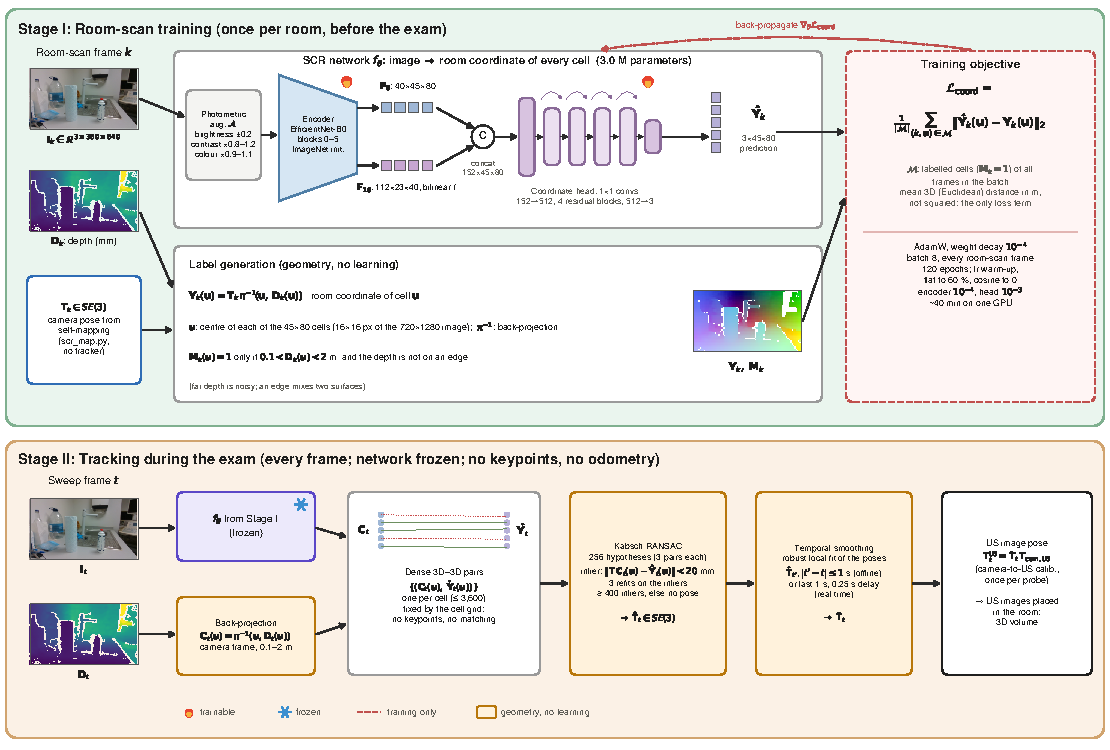
\includegraphics[width=0.90 \linewidth]{fig_architecture.pdf} 
  \caption{Network, labels and pose solver. Training (once per room): each room-scan frame $I_k$ passes through the network; its depth $D_k$ and self-mapped pose $T_k$ give the label $Y_k(\mathbf{u})$ of every valid cell, and the loss is the mean 3D distance between prediction and label (Eq.~\eqref{eq:loss}). Pose estimation (every examination frame): the network gives a room point $\hat{\mathbf{y}}_i$ per cell and the measured depth the same cell in the camera frame, $\mathbf{x}_i$; these dense 3D--3D pairs, fixed by the cell grid, are aligned by Kabsch RANSAC (Eq.~\eqref{eq:kabsch}).}
  \label{fig:architecture}
\end{figure*}

\subsection{Training Labels and Loss}
\label{sec:training}
Given pose $T_k$, the label of cell $\mathbf{u}$ is its depth point placed in the room, $Y_k(\mathbf{u})=T_k\,\pi^{-1}(\mathbf{u},D_k(\mathbf{u}))$. A cell is labelled only if $0.1\,\mathrm{m}<D_k(\mathbf{u})<2$\,m and no neighbouring cell is more than 6\,\% nearer or farther (a depth edge mixes two surfaces). The loss is the mean Euclidean distance over the labelled cells $\mathcal{M}$ of a batch,
\begin{equation}
  \mathcal{L}(\theta)=\frac{1}{|\mathcal{M}|}\sum_{(k,\mathbf{u})\in\mathcal{M}}\left\|f_\theta(I_k)(\mathbf{u})-Y_k(\mathbf{u})\right\|_2 .
  \label{eq:loss}
\end{equation}
The distance is not squared, so the gradient does not vanish as the error approaches the millimetre scale. One network is trained per room on all its room-scan frames with AdamW (learning rate $10^{-3}$ for the head and $10^{-4}$ for the encoder, weight decay $10^{-4}$, batch size 8) for 120 epochs, with a constant rate for 60\,\% of the steps and a cosine decay to zero; 40 epochs give the same accuracy (Sec.~\ref{sec:res_main}). Augmentation is photometric only (brightness $\pm0.2$, contrast 0.8--1.2, per-channel gain 0.9--1.1). One epoch passes once over all room-scan frames in random order (\textcolor{red}{iterations per epoch for S-test} iterations for \Stest{}); the encoder runs in \textcolor{red}{mixed / single} precision. The same loss and settings are used inside self-mapping (Sec.~\ref{sec:mapping}), where each round trains for a fixed number of steps; between rounds the network is \textcolor{red}{continued / re-initialised}, and the final network is trained \textcolor{red}{from scratch / fine-tuned from the last round} on the labels of the optimised poses.

\subsection{Per-Frame Pose Estimation}
\label{sec:pose}
Every cell $i$ with depth $d_i<2$\,m gives a camera point $\mathbf{x}_i=\pi^{-1}(\mathbf{u}_i,d_i)$ and a predicted room point $\hat{\mathbf{y}}_i=f_\theta(I)(\mathbf{u}_i)$; the correspondences are fixed by the cell grid, without keypoints or descriptors. For a set $\mathcal{S}$, the Kabsch fit \cite{kabsch1976}
\begin{equation}
  (R,\mathbf{t})=\arg\min_{R\in SO(3),\,\mathbf{t}}\ \sum_{i\in\mathcal{S}}\|R\mathbf{x}_i+\mathbf{t}-\hat{\mathbf{y}}_i\|^2
  \label{eq:kabsch}
\end{equation}
has a closed-form solution by singular value decomposition. The inliers of a pose are $\mathcal{I}=\{i:\|R\mathbf{x}_i+\mathbf{t}-\hat{\mathbf{y}}_i\|<20\,\mathrm{mm}\}$. RANSAC \cite{fischler1981ransac} draws 256 samples of three correspondences, keeps the hypothesis with most inliers, and refits it three times on its inliers, re-evaluating the inlier set after each refit, giving the pose $\hat T_t$ and inlier count $n_t$ (at most 3600, the number of cells). The three cells of a sample are drawn \textcolor{red}{uniformly from the valid cells / other rule}; degenerate samples (e.g.\ nearly collinear points) are handled by \textcolor{red}{check and threshold}. Frames with $n_t<400$ receive no pose (the \emph{inlier gate}). No earlier pose is used as a prior, so errors cannot accumulate over a sweep.

\subsection{Self-Mapping Without a Tracker}
\label{sec:mapping}
Self-mapping estimates all $T_k$ from the RGB-D room scan alone (Algorithm~\ref{alg:mapping}), with the loss of Sec.~\ref{sec:training} and the pose estimation of Sec.~\ref{sec:pose}; several videos are mapped jointly into one frame.

The seed frame defines $W$; the first try is \textcolor{red}{first frame of the first video / other rule}. Frames within $\pm2$\,s of it are placed by frame-to-frame point-to-plane ICP on the depth \cite{chen1992icp,TODO-low2004} (points on a 4-pixel grid, inlier distance 10\,mm; accepted if $\ge50$\,\% inliers with RMS $\le6$\,mm), chaining the relative poses outwards from the seed. ICP is implemented with \textcolor{red}{library} and runs for at most \textcolor{red}{iterations} iterations from \textcolor{red}{initial guess: identity / previous relative motion}. If ICP places less than 1\,s of the scan, e.g.\ because a hand covers the camera, the seed moves 1\,s later, up to 20 times; if no try succeeds, the best one is used.

Each round trains the network on the placed frames (2000 steps in the first round, 1500 afterwards) and localises the others with it. A frame within 150 frames of a placed frame of the same video joins if it has $\ge60$ inliers and its implied motion is plausible: its pose differs from that of the nearest placed frame of the same video, $\Delta t$ apart, by at most $500\,\mathrm{mm/s}\cdot\Delta t+20$\,mm in position and $90^\circ/\mathrm{s}\cdot\Delta t+5^\circ$ in orientation; every 30th remaining frame joins if it has $\ge400$ inliers, which admits a second video. Depth ICP then extends each placed segment by up to 90 frames at both ends. Mapping stops when a round adds fewer than 0.5\,\% of the frames (\textcolor{red}{typical number of rounds} rounds in our sessions; on \Stest{}, 92\,\% of the frames were placed after the first round and all after the second); a final pass relocalises every frame and keeps poses with $\ge400$ inliers as initial poses $T^0_k$.

Independently localised frames are individually plausible, but the map bends over seconds. The graph combines the network poses with ICP relative poses $Z_{ij}$: \emph{sequential} edges between frames 1, 5, 15 and 30 apart, and \emph{loop-closure} edges between frames more than 2\,s apart or from different videos that observe the same part of the room (for every third frame, up to three partners whose camera centres and points 1\,m ahead both lie within 150\,mm). Each $Z_{ij}$ is estimated by the point-to-plane ICP above, initialised with \textcolor{red}{the relative pose of the network poses / identity}. Edges whose $Z_{ij}$ deviates from the map by more than 50\,mm are dropped. With $T_k=T^0_k\,\mathrm{Exp}(\boldsymbol{\delta}_k)$, four points $Q$ 1\,m in front of the camera, and $P=Q\cup\{\mathbf{0}\}$, the graph minimises
\begin{equation}
  \begin{aligned}
  &\sum_{(i,j)}\sum_{\mathbf{p}\in P}\rho\!\left(\frac{\|Z_{ij}^{-1}T_i^{-1}T_j\mathbf{p}-\mathbf{p}\|^2}{\sigma_e^2}\right)\\
  &\quad+\sum_{k}\sum_{\mathbf{q}\in Q}\rho\!\left(\frac{\|T_k\mathbf{q}-T^0_k\mathbf{q}\|^2}{\sigma_p^2}\right)
  \end{aligned}
  \label{eq:posegraph}
\end{equation}
over $\{\boldsymbol{\delta}_k\}$, with $\sigma_e=1$\,mm, $\sigma_p=10$\,mm and $\rho(z)=2(\sqrt{1+z}-1)$, using \textcolor{red}{solver, e.g. Levenberg--Marquardt / trust-region least squares} for at most \textcolor{red}{iterations} iterations. Point residuals put all constraints in millimetres without a rotation weight, and the points ahead constrain orientation through what the camera sees. The prior fixes the gauge and keeps ICP failures from bending the map. The optimised poses label the final network (Sec.~\ref{sec:training}).

\begin{algorithm}[t]
  \caption{Self-mapping of a room scan}
  \label{alg:mapping}
  \small
  \begin{algorithmic}[1]
    \Require RGB-D room scan $\{(I_k,D_k)\}_{k=1}^{N}$
    \Ensure poses $\{T_k\}$ in the map frame $W$
    \State choose seed $k_0$; $T_{k_0}\gets I$; place frames within $\pm2$\,s by depth ICP
    \If{less than 1\,s placed} move $k_0$ 1\,s later and repeat (max.\ 20 tries) \EndIf
    \State $\mathcal{P}\gets$ placed frames; $n\gets2000$
    \Repeat
      \State train $f_\theta$ on $\mathcal{P}$ for $n$ steps (Eq.~\eqref{eq:loss}); $n\gets1500$
      \State localise every $k\notin\mathcal{P}$ (Sec.~\ref{sec:pose})
      \State add $k$ near $\mathcal{P}$ with $\ge60$ inliers and plausible motion
      \State add every 30th remaining $k$ with $\ge400$ inliers
      \State extend each segment of $\mathcal{P}$ by depth ICP (up to 90 frames)
    \Until{fewer than 0.5\,\% of the frames added}
    \State $T^0_k\gets$ relocalise all frames; keep if $\ge400$ inliers
    \State build sequential and loop-closure ICP edges; drop edges off by $>50$\,mm
    \State \Return $\{T_k\}\gets$ solution of Eq.~\eqref{eq:posegraph}
  \end{algorithmic}
\end{algorithm}

\subsection{Hand--Eye and Ultrasound Calibration, Synchronisation}
\label{sec:sensorcal}
The two fixed calibrations in Eq.~\eqref{eq:chain} come from the optical tracker and are needed once per probe. The marker-to-camera hand--eye calibration $T^M_C$ is estimated from \textcolor{red}{number} views of a \textcolor{red}{calibration board type} observed by the camera while the tracker records the marker, by \textcolor{red}{method, e.g. AX=XB solver}; its error is 3.5\,mm at the corners of the board. The marker-to-image calibration $T^M_U$ is obtained with \textcolor{red}{phantom and method} \textcolor{red}{reference}, with a residual of \textcolor{red}{value}\,mm. Camera, US and tracker frames are time-stamped by \textcolor{red}{common clock / per-device clocks}, and the streams are matched by \textcolor{red}{nearest timestamp / interpolation of the tracker poses}; a residual offset is checked as in Sec.~\ref{sec:data}.

\subsection{Probe Calibration}
\label{sec:calib}
With a tracker, the camera pose is measured through the hand--eye calibration, $T^{\mathrm{trk}}_k=T^{\mathrm{trk}}_M(k)\,T^M_C$, so an error of $T^M_C$ shifts the camera frame by a fixed transform. For a map built from tracker poses, this error cancels, because labels, ground truth and $T^C_U$ refer to the same displaced frame. A self-made map refers to the physical camera, so the error appears as a fixed offset between the map and $T^C_U$. We model it by $X$ and estimate it jointly with the alignment $A$ of $W$ to the tracker frame over the room-scan frames,
\begin{equation}
  (A,X)=\arg\min_{A,X}\sum_k\sum_{\mathbf{q}\in P}\rho\big(\|A\,T_k\,X\,\mathbf{q}-T^{\mathrm{trk}}_k\mathbf{q}\|\big).
  \label{eq:calib}
\end{equation}
We minimise Eq.~\eqref{eq:calib} over \textcolor{red}{all / every n-th} room-scan frame with a tracker pose, with a soft-L1 loss of scale 5\,mm, starting from ten alternating steps ($A$ by a Kabsch fit, $X$ as the mean transform), with $P$ the camera centre and the four points of Eq.~\eqref{eq:posegraph}. $X$ is a property of the probe: it is fitted once on the room scans of \Stest{} and reused unchanged on \Snew{} and \Sctrl{}. In deployment, a phantom calibration would replace the tracker. $A$ is used for evaluation only, because $W$ is arbitrary.

\subsection{Temporal Smoothing}
\label{sec:smoothing}
For frame $t$ at time $s_t$, the poses $j$ in a window with $\Delta_j=s_j-s_t$ are weighted by $w_j=n_j(1-|\Delta_j/h|^3)^3$, where $n_j$ is the inlier count and $h$ the half-width of the window. Translations are fitted by a weighted polynomial in $\Delta_j$, quadratic if at least five poses surround $s_t$, linear with three or four, constant otherwise, and rotations, as rotation vectors about the weighted mean rotation, in the same way. Two Tukey reweightings make the fit robust: a pose is down-weighted by $(1-(r_j/c)^2)^2$, where $r_j$ adds the translation residual in mm and 0.16\,mm per mrad of rotation residual (the lever arm to the image), and $c$ is six times the median residual. Offline, the window is centred, $|\Delta_j|\le1$\,s. In real time, the pose of frame $t$ is output 0.25\,s later from the last 1\,s of poses, $\Delta_j\in[-0.75,0.25]$\,s, extrapolated linearly to $s_t$; the fully causal variant uses the last 0.25\,s, $\Delta_j\in[-0.25,0]$\,s. Both windows were chosen on \Sval{} as the lowest error for their delay.

\subsection{3D Compounding}
\label{sec:compounding}
Each US pixel is placed in $W$ by Eq.~\eqref{eq:chain} with the smoothed pose $\bar T_t$ and accumulated in a voxel grid of \textcolor{red}{voxel size}\,mm, aligned with \textcolor{red}{the map frame / the first image of the sweep}. Pixels falling into the same voxel are combined by \textcolor{red}{mean / maximum / last value}, and empty voxels are \textcolor{red}{left empty / filled by interpolation within a distance}. Reference volumes are compounded in the same way from the tracker poses. For display, a slab of \textcolor{red}{thickness}\,mm around \textcolor{red}{plane} is projected by \textcolor{red}{maximum / mean} along the viewing direction.

\subsection{Room-Scan Protocol and Pre-Examination Checks}
\label{sec:protocol}
The experiments (Sec.~\ref{sec:res_coverage}--\ref{sec:res_changes}) motivate three steps of the procedure; they were not tuned as components. (a)~\emph{Exam-view scan:} the operator records the room scan with the probe held in the air along each planned sweep path, at sweep height and angle. (b)~\emph{Coverage check:} after the first sweep, the share of sweep frames with a room-scan pose within 30\,mm (camera centre) and $10^\circ$ (orientation) is computed, searching all room-scan poses for each sweep frame; the examination proceeds if it is at least 80\,\%. In this study the check uses the tracker; a tracker-free version, comparing the tracked poses with the self-mapped scan poses, is future work. (c)~\emph{Map-age check:} the median Kabsch inlier count $n_t$ over the frames of a session flags an outdated map, in which case the room is rescanned; in this study the median was computed over \textcolor{red}{all sweep frames of the session / the first sweep}.

\subsection{Design Choices}
\label{sec:design}
The pose comes from exact geometry on learned correspondences rather than from a learned pose, because pose regression was about $8\times$ less accurate in our setting (Sec.~\ref{sec:res_compare}). No temporal model is learned: odometry added nothing once every frame has an absolute pose, and a fixed robust smoother reduces the jitter (Sec.~\ref{sec:res_ablation}). Poses are refined by the pose graph only, not jointly with the network as in ACE0, because joint refinement made an \Stest{} map less accurate (camera position 8.4 to 8.9\,mm).




%======================================================================
\section{Experiments}
\label{sec:experiments}
%======================================================================

\subsection{Set-Up and Ground Truth}
\label{sec:data}\label{sec:implementation}\label{sec:groundtruth}
A RealSense D435i (colour $1280\times720$ at about 30\,Hz, depth aligned to colour) was mounted on a linear probe \tbd{probe and scanner model}. The US image was grabbed from the scanner ($640\times480$, 0.23\,mm/px, 9\,cm depth, 19 frames/s). An NDI Polaris Vega tracked a marker on the probe; the hand--eye calibration has 3.5\,mm error at the calibration-board corners. Streams were synchronised offline; comparing the self-made map with the tracker showed no residual timing offset (best shift $+3$ to $+9$\,ms). Sweeps were acquired on the forearm of two subjects and on a phantom \tbd{phantom type; ethics approval}.

The method is implemented in PyTorch and runs on one NVIDIA RTX A4500 GPU. Self-mapping takes about 30\,min per room and training the final network about 40\,min for 120 epochs (13\,min for 40). ORB-SLAM3 runs on the CPU of the same computer. \tbd{code availability}

In every session the probe marker was at the near edge of the tracker's measurement volume (median distance 0.88--0.93\,m); the tracker noise at the US image was 0.12--0.25\,mm, and our error showed no trend with the marker distance (supplementary material). The reference is the same in all sessions, so a bias common to all of them cannot be excluded.

\subsection{Sessions and Protocol}
\label{sec:sessions}\label{sec:rules}
All sessions were recorded in the same room (Table~\ref{tab:sessions}). \emph{\Sval{}} is used only for validation. \emph{\Stest{}}, later the same day with a few objects moved, is the test session. \emph{\Snew{}}, five days later, has five blocks: A new session, B small room change, C large room change, D second subject, E arm in view of the camera; its room scans are short and generic. \emph{\Sctrl{}} is a controlled session on a phantom, with five blocks: A reference, B large rearrangement, C very large rearrangement, D people moving in the background (C's layout and scans), E emptied room. Each \Sctrl{} block has two room scans: a \emph{generic} scan, walking the room, and an \emph{exam-view} scan, the probe held in the air along each of the four sweep paths (views) at sweep height and angle. In total, 65 sweeps are evaluated: 2 for validation and 63 for testing.

\begin{table}[t]
  \caption{Sessions, all in one room. Coverage: share of sweep frames with a room-scan pose within 30\,mm and $10^\circ$ (mean over sweeps).}
  \label{tab:sessions}
  \centering
  \scriptsize
  \setlength{\tabcolsep}{2.5pt}
  \begin{tabular}{@{}lllcll@{}}
    \toprule
    Session & Date & Subject & Sweeps & Room scans & Role / coverage\\
    \midrule
    \Sval & 9 Oct & forearm & 2 & 3.0\,min & validation\\
    \Stest & 9 Oct & forearm & 5 & 2.0\,min & test; 93--96\,\%\\
    \Snew & 14 Oct & forearm, 2 subj. & 26 (5 blocks) & 40--90\,s, generic & test; 0--14\,\%\\
    \Sctrl & 5 Nov & phantom & 32 (5 blocks) & exam-view + generic & controlled test\\
    \bottomrule
  \end{tabular}
\end{table}

All settings were chosen on \Sval{}; nothing was tuned on the test sessions. $X$ was fitted on \Stest{} and reused unchanged. Before the \Sctrl{} analysis we fixed that the exam-view scan is the protocol and gives each block's headline number, and that the generic scans and earlier blocks' scans are controlled tests. Each network is trained on its block's room scan only. As an additional test of maps that contain objects moved since, \Snew{} networks were also trained on all room scans of the day up to the block (\emph{pooled}); this variant was examined on the test blocks and is reported in the supplementary material, not as part of the method. Seed spread was measured with three training seeds on \Stest{} and on every \Sctrl{} block. To compare with ORB-SLAM3 we pair the systems by sweep and report the mean difference with a 95\,\% bootstrap interval and a Wilcoxon signed-rank test. As a check that the tracker does not reach the reported numbers through the smoothing, we also smoothed every sweep as one piece instead of restarting at the breaks caused by tracker dropouts; the results were identical to two decimals on all splits.

\subsection{Experiments}
\label{sec:baselines}\label{sec:ablations}\label{sec:occlusion}
The Results follow five experiments, in the same order.

\emph{1) Accuracy with a covering room scan} (Sec.~\ref{sec:res_main}). Our system is evaluated on \Stest{} and on the exam-view scans of \Sctrl{}, against the \emph{oracle map}, the same network trained on tracker poses of the room scan, which isolates mapping from tracking. On \Stest{} we also use only the room scan recorded before the sweeps (\emph{strict protocol}) and the real-time and causal smoothing; we repeat training with three seeds and, on \Sctrl{} A, with 20 to 120 epochs.

\emph{2) Ablations} (Sec.~\ref{sec:res_ablation}). Self-mapping is repeated from scratch without loop closures and without the probe calibration $X$. The tracking settings are varied on \Sval{} with the oracle map (training length, PnP instead of Kabsch, geometric augmentation, input resolution, smoothing). The \emph{hybrid} uses our per-frame poses once per second as anchors in a SIFT odometry with a pose graph, and \emph{odometry only} poses each segment start with the tracker. $X$ is fitted on each \Stest{} scan alone and refitted on \Snew{} C as a diagnostic.

\emph{3) Room scan and scene changes} (Sec.~\ref{sec:res_coverage}). On \Sctrl{}, the same sweeps are tracked with the exam-view scan, the generic scan, both scans in one map, and an earlier block's map (\emph{outdated}); per frame, we relate the anchor error to the distance to the nearest room-scan pose, and on \Stest{} we map the first 20, 40 and 60\,s of the scans. \Snew{}, with short generic scans, is the uncontrolled case.

\emph{4) Baselines} (Sec.~\ref{sec:res_compare}). \emph{Classical pipeline:} once per second, SIFT \cite{lowe2004sift} matches (4000 features, ratio 0.8) against the three room-scan keyframes nearest to the current pose, lifted to 3D with depth and solved by PnP-RANSAC \cite{lepetit2009epnp} (4\,px); SIFT RGB-D odometry in between and a pose graph combine them \cite{TODO-classical-pipeline}. Its keyframe poses come from the tracker; we also run it on our tracker-free map. \emph{Pose regression:} a network that regresses the pose between a keyframe and the query, with learned odometry \cite{TODO-own-pose-regression}. \emph{US only:} the method of Li et al.\ \cite{li2024longterm}.

\emph{ORB-SLAM3} \cite{campos2021orbslam3} in RGB-D mode with its default ORB vocabulary, 1250 ORB features on 8 pyramid levels (scale factor 1.2), viewer off, playing each sequence in real time \tbd{ORB-SLAM3 version (commit)}. Each session is exported as one sequence: the room scan(s), then the sweeps. We run it in three modes. \fullslam{}: it maps the room scan and keeps mapping during the sweeps, with loop closing. \loconly{}: it maps the room scan, after which mapping is switched off, so the sweeps are tracked against a frozen room-scan map, the information our system has. \reloc{}: as localisation only, but before every sweep frame the tracking state is reset, so each frame is relocalised against the frozen map with nothing from the previous frame, the task our network solves. In localisation mode, ORB-SLAM3 relocalises only after it has declared the camera lost, which in this mode never happens; we changed one line so that it relocalises as soon as tracking fails. We score the poses \emph{as tracked}, i.e.\ as a live system would show them, and for full SLAM also the trajectory \emph{refined at shutdown}. The alignment and ORB-SLAM3's own probe calibration are fitted on the room-scan frames only, as for ours; its \Stest{} calibration is reused on the other sessions; poses are smoothed over 1\,s; frames not tracked count as without a pose.

\emph{5) Controlled occlusion} (Sec.~\ref{sec:res_occlusion}). To test how each system degrades when part of the view is blocked, as by the operator's hand or arm, we added a synthetic occluder to the sweep frames of \Sctrl{} B and C (16 sweeps). It is a band over the full image height and 30\,\% or 60\,\% of the image width, filled with a skin-like colour and a fixed texture, so that keypoint detectors find corners on it, at a depth of 0.4\,m. It appears for 3\,s every 10\,s, starting 5\,s into each sweep and alternating between the left and right side, so that about 30\,\% of the sweep time is occluded. The room scans are not occluded. Both systems receive identical frames.

\subsection{Metrics}
\label{sec:metrics}
Errors are measured at the US image, about 16\,cm from the camera, at 5 points spanning the image (\textcolor{red}{e.g. the four corners and the centre of the imaged region}); we report the median per sweep and the mean over sweeps. \emph{Absolute:} after one rigid alignment $A$ per session, never per sweep. \emph{Shape:} after the best rigid fit of each sweep; it measures the distortion of the reconstructed volume. \emph{Worst sweep:} the largest per-sweep median of a split, reported where single sweeps fail. \emph{Relative motion:} out-of-plane error of the relative pose between frames 8 or 30 rows apart. \emph{Jitter:} mean change of the error over 8 frames (0.27\,s). \emph{Anchors:} camera-position error of single-image localisation, once per second, used to compare localisers without smoothing or odometry. \emph{Posed:} share of sweep frames with a pose. \emph{Coverage:} as in Table~\ref{tab:sessions}. \emph{Map error:} camera-centre error of the room-scan poses against the tracker after one alignment; for \Stest{} also the points 1\,m in front of the camera, the orientation and the relative motion over 1\,s.

%======================================================================
\section{Results}

\subsection{Tracking With a Covering Room Scan}
\label{sec:res_main}
On \Stest{} (Table~\ref{tab:test}), our system reaches 2.34\,mm absolute and 1.72\,mm shape error; three training seeds give 2.22--2.34\,mm (mean 2.27\,mm). The oracle map reaches 1.85 / 1.57\,mm (seeds 1.85, 1.95 and 2.12\,mm), 0.49\,mm lower. The classical pipeline reaches 3.11 / 2.47\,mm and odometry alone 9.43 / 6.23\,mm. ORB-SLAM3 tracked every frame in every mode and reached 1.72--1.84\,mm absolute and 1.18--1.38\,mm shape. The out-of-plane error over 8 rows is 0.23--0.37\,mm for all systems. Under the strict protocol, our error is 2.94\,mm (oracle map 2.98, classical 3.0\,mm). Real-time smoothing with 0.25\,s delay gives the offline result (2.34\,mm), and fully causal smoothing 2.42\,mm. On \Sctrl{} with the exam-view scans (Table~\ref{tab:ctrl}), blocks A, C and D give 2.28, 3.11 and 2.24\,mm (shape 1.70--1.90\,mm), and block A with the oracle map 1.85\,mm. Three seeds per \Sctrl{} block differ by 0.03--0.27\,mm (A $2.26\pm0.03$, B $4.20\pm0.23$, C $3.17\pm0.12$, D $2.22\pm0.03$, E $6.00\pm0.27$\,mm). On \Sctrl{} A, 20 / 40 / 80 / 120 training epochs give 2.53 / 2.34 / 2.37 / 2.28\,mm.

\begin{table*}[t]
  \caption{\Stest{} (5 sweeps), error at the US image (mm): absolute, shape, out-of-plane error of the relative pose over 8 / 30 rows, and jitter. Real time: 0.25\,s delay. Tracker: what each system takes from the tracker besides evaluation. ORB-SLAM3 poses are smoothed over 1\,s, ours over 2\,s on \Stest{} (1\,s gives 2.36\,mm). Lower part: self-mapping ablations. Bold: best per column.}
  \label{tab:test}
  \centering
  \scriptsize
  \setlength{\tabcolsep}{3pt}
  \begin{tabular}{@{}llcccccc@{}}
    \toprule
    System & Tracker & Abs. & Shape & Out-of-pl.\ 8 / 30 & Jitter & Posed\\
    \midrule
    Ours, self-mapped & calib.\ $X$ & 2.34 & 1.72 & 0.37 / 0.62 & 0.90 & 100\,\%\\
    \quad strict protocol & calib.\ $X$ & 2.94 & -- & -- & -- & \NQ\\
    \quad real time / causal & calib.\ $X$ & 2.34 / 2.42 & -- & -- & -- & 100\,\%\\
    ORB-SLAM3, full SLAM, refined at shutdown & own calib. & 1.79 & 1.34 & 0.25 / 0.45 & 0.73 & 100\,\%\\
    ORB-SLAM3, full SLAM, as tracked & own calib. & 1.81 & \textbf{1.18} & \textbf{0.23} / \textbf{0.38} & \textbf{0.67} & 100\,\%\\
    ORB-SLAM3, localisation only & own calib. & 1.84 & 1.30 & 0.25 / 0.43 & 0.68 & 100\,\%\\
    ORB-SLAM3, each frame relocalised & own calib. & \textbf{1.72} & 1.38 & 0.26 / 0.44 & 0.76 & 100\,\%\\
    Oracle map & map poses & 1.85 & 1.57 & 0.37 / 0.62 & 0.93 & 100\,\%\\
    Classical anch.\ + odom. & keyframes & 3.11 & 2.47 & 0.29 / 0.62 & 1.09 & \NQ\\
    Classical odom.\ only & seg.\ start & 9.43 & 6.23 & 0.28 / 0.54 & -- & \NQ\\
    \midrule
    \multicolumn{7}{@{}l}{\emph{Self-mapping ablations (mapped from scratch, one component removed)}}\\
    Ours without loop closures & calib.\ $X$ & 5.77 & 3.18 & -- & -- & \NQ\\
    Ours without calibration $X$ & none & 11.49 & 4.08 & -- & -- & \NQ\\
    \bottomrule
  \end{tabular}
\end{table*}

\subsection{Ablations}
\label{sec:res_ablation}\label{sec:res_mapping}\label{sec:res_tracking}\label{sec:res_calib}
Self-mapping placed all 3356 \Stest{} room-scan frames (92\,\% after the first round, 100\,\% after the second). Against the tracker, the map has 2.6\,mm error at points 1\,m in front of the camera, 2.0\,mm at the camera centre, $0.19^\circ$ in orientation and 1.5\,mm in relative motion over 1\,s. Without loop closures, the error at the US image rises from 2.34 / 1.72 to 5.77 / 3.18\,mm, and without the probe calibration $X$ to 11.49 / 4.08\,mm (Table~\ref{tab:test}, lower part).

With the oracle map on \Sval{}, 120 instead of 15 training epochs reduced the anchor error from 15.8 to 5.1\,mm, and Kabsch with depth instead of PnP to 3.4\,mm; geometric augmentation and full-resolution input raised it (3.4 to 6.5\,mm; 6.3 to 7.3\,mm). On \Stest{}, smoothing reduced the jitter from 1.67 to 0.93\,mm and the error at the US image from 2.03 to 1.85\,mm. The hybrid gives 6.54\,mm on \Snew{}, against 6.48\,mm without odometry, and learned odometry is 0.3--0.6\,mm worse.

Fitted on each \Stest{} scan alone, $X$ agrees within 1.8\,mm and $0.05^\circ$, and each fit is valid on the other scan (scene points 2.9\,mm). Fitted on \Snew{}, its rotation differs by about $0.5^\circ$; refitting $X$ on \Snew{} C lowers the error in C from 9.40 to 7.87\,mm and in D from 11.54 to 9.58\,mm.

\subsection{Room Scan and Scene Changes}
\label{sec:res_coverage}\label{sec:res_changes}
\emph{Coverage.} On the same 8 \Sctrl{} A sweeps (Table~\ref{tab:ctrl}), the exam-view scan (96\,\% coverage) gives 2.28 / 1.90\,mm with our map and 1.85 / 1.67\,mm with the oracle map; the generic scan (0\,\%) gives 13.57 / 3.79 and 10.95 / 3.93\,mm. With the generic map the volume is displaced but keeps its shape (Fig.~\ref{fig:volume}), and every frame passed the inlier gate. Both scans in one map give 3.15 / 1.81\,mm, with a map camera error of 3.4 instead of 2.7\,mm. Over all current \Sctrl{} maps (Fig.~\ref{fig:coverage_error}), our shape error is 1.28--3.79\,mm, and with at least 90\,\% coverage the absolute error is about the map camera error plus 1\,mm. The exam-view scan gives the lower error in every block except B, where it covered 75\,\% and the generic scan 93\,\% (4.43 vs.\ 3.36\,mm). The emptied room E gives the largest map errors (4.3 and 10.9\,mm). Per frame, with the oracle map, the anchor error is 4.1\,mm for sweep frames within 30\,mm and $10^\circ$ of a room-scan pose and 13.4\,mm for the others, and the first 20 / 40 / 60\,s of each \Stest{} scan give 3.00 / 2.03 / 1.85\,mm (further views in the supplementary material).

\begin{table*}[t]
  \caption{\Sctrl{}, current maps (upper part) and outdated maps (lower part). Error at the US image (mm), absolute / shape; coverage; camera error of the map (mm). Exam-view scans are the protocol (headline per block); generic scans are a controlled test. ORB-SLAM3: localisation only (map from the same room scan, then frozen). Outdated maps: views covered 84--96\,\% overall; median Kabsch inliers in Sec.~\ref{sec:res_changes}. For ORB-SLAM3, B's outdated map is built from B's generic scan, as for ours.}
  \label{tab:ctrl}
  \centering
  \scriptsize
  \setlength{\tabcolsep}{6pt}
  \begin{tabular}{@{}llccccc@{}}
    \toprule
    Block & Room scan & Cov. & Map & Ours & Oracle & ORB-SLAM3\\
    \midrule
    A reference & \textbf{exam-view} & 96\,\% & 2.7 & \textbf{2.28 / 1.90} & 1.85 / 1.67 & 3.79 / 1.34\\
     & exam-view, after sweeps & -- & 2.0 & 2.50 / 1.96 & -- & --\\
     & generic & 0\,\% & 6.5 & 13.57 / 3.79 & 10.95 / 3.93 & 2.88 / 1.19\\
     & both in one map & \NQ & 3.4 & 3.15 / 1.81 & -- & --\\
    B large change & \textbf{exam-view} & 75\,\% & 2.4 & \textbf{4.43 / 2.81} & -- & 1.70 / 1.17\\
     & generic & 93\,\% & 2.2 & 3.36 / 2.46 & -- & --\\
    C very large & \textbf{exam-view} & 96\,\% & 2.2 & \textbf{3.11 / 1.76} & -- & 2.05 / 1.11\\
     & generic & 78\,\% & 5.2 & 6.35 / 1.76 & -- & --\\
    D people moving & \textbf{exam-view} & 98\,\% & 2.2 & \textbf{2.24 / 1.70} & -- & 1.60 / 1.74\\
     & generic & 100\,\% & 5.2 & 5.07 / 1.28 & -- & --\\
    E empty room & \textbf{exam-view} & 92\,\% & 4.3 & \textbf{5.85 / 3.04} & -- & 2.65 / 0.99\\
     & generic & 97\,\% & 10.9 & 13.03 / 2.83 & -- & --\\
    \midrule
    \multicolumn{7}{@{}l}{\emph{Outdated maps: an earlier block's map on a later block's sweeps}}\\
    B large change & A's map & \NQ & -- & 4.28 / 3.00 & -- & --\\
    C very large & A's map & \NQ & -- & 59.4 (21\,\% posed) & -- & --\\
    C very large & B's map & \NQ & -- & 40.9 (96\,\% posed) & -- & 19.19 / 10.58$^{a}$\\
    E empty room & C's map & \NQ & -- & 13.9 (p90 46.6) & -- & 4.19 / 2.51\\
    \bottomrule
  \end{tabular}\\[2pt]
  \raggedright\footnotesize $^{a}$Sweeps 5--8 only; sweeps 1--4 were not tracked.
\end{table*}

\begin{figure}[t]
  \centering
  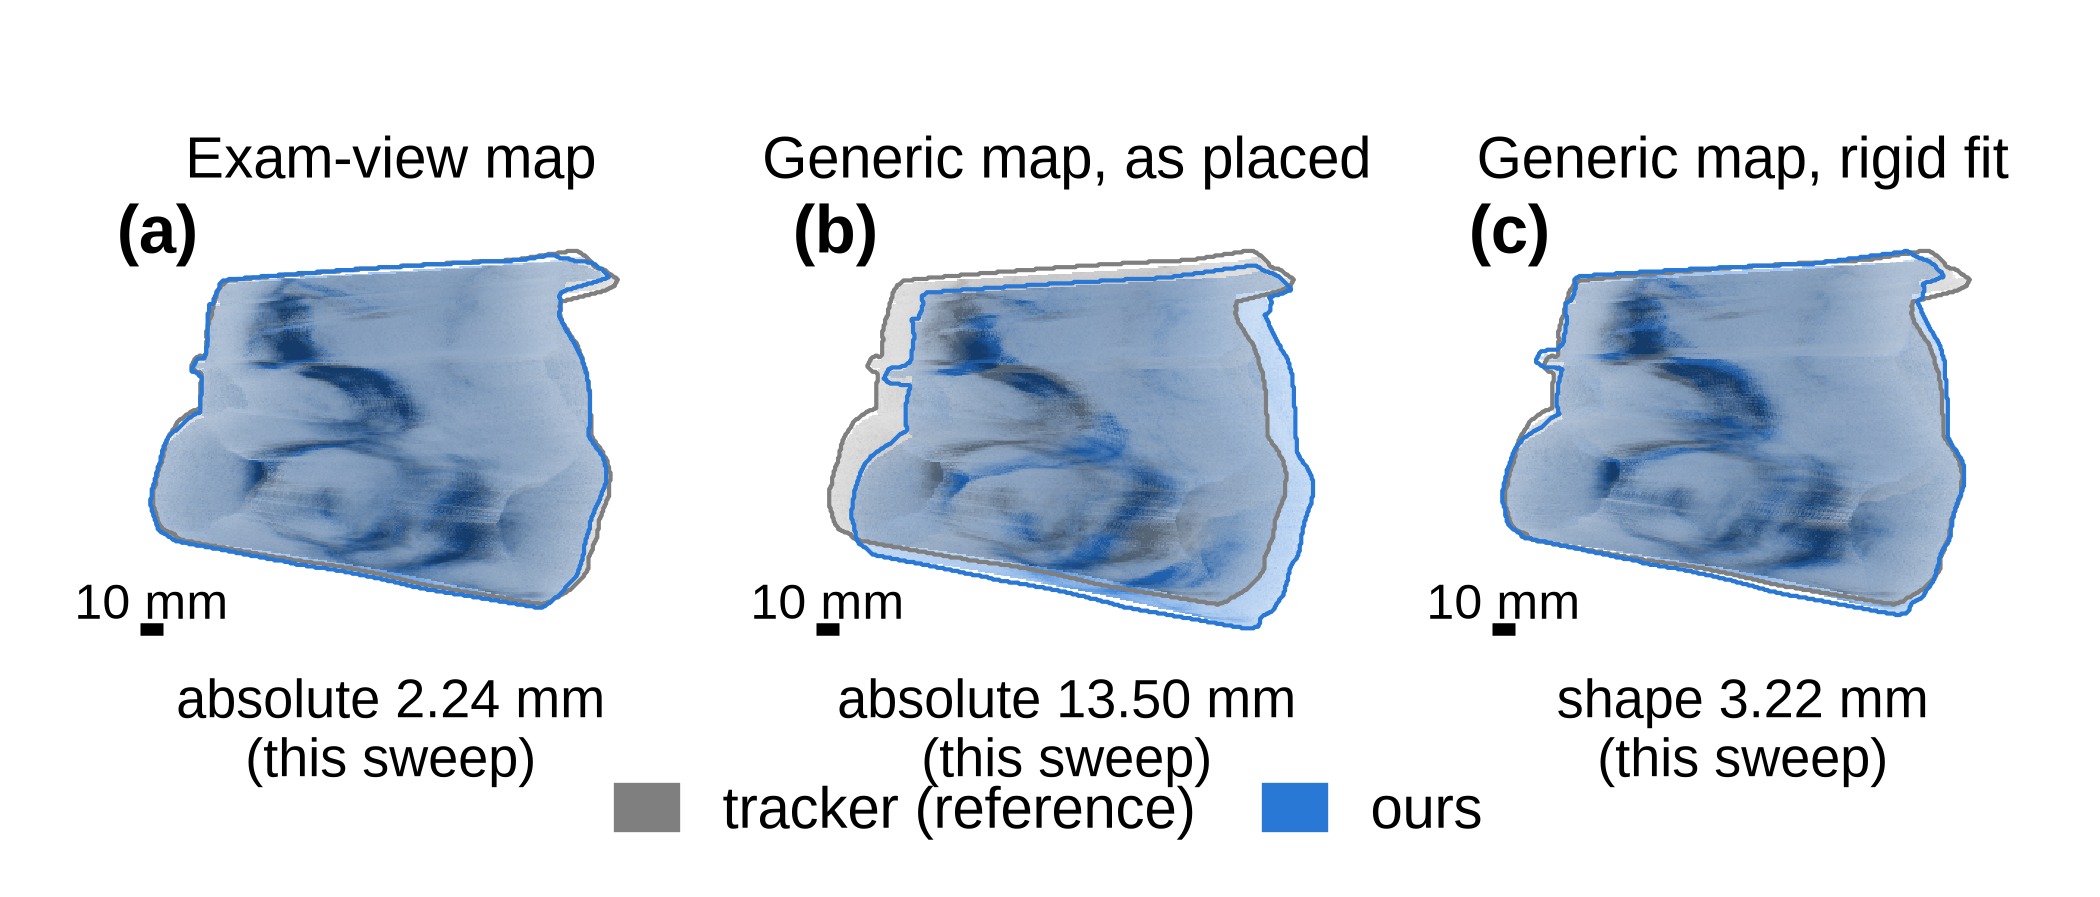
\includegraphics[width=0.90 \linewidth]{fig_volume_coverage.png} 
  \caption{One \Sctrl{} A sweep compounded with the tracker poses (grey) and with ours (blue), slab projection seen from the skin; outlines: footprint of each volume; multiply blend, so dark where both agree. (a)~Exam-view map, as placed: 2.24\,mm. (b)~Generic map, which misses the examination views, as placed: 13.50\,mm. (c)~Generic map after the best rigid fit of the sweep: 3.22\,mm. The generic map misplaces the volume but keeps its shape. Values for this sweep; block means 2.28 / 1.90 and 13.57 / 3.79\,mm.}
  \label{fig:volume}
\end{figure}

\begin{figure}[t]
  \centering
  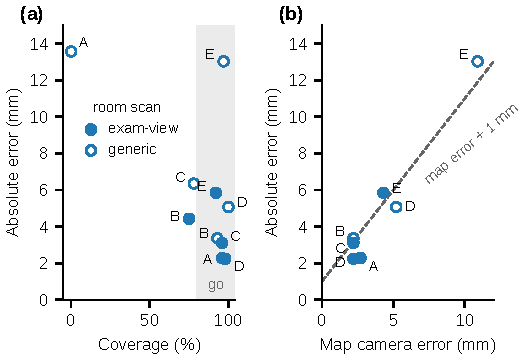
\includegraphics[width=0.90 \linewidth]{fig_coverage_error.pdf}
  \caption{\Sctrl{} maps, one point per block and room scan (filled: exam-view scan; open: generic scan). (a)~Error at the US image against coverage of the sweep viewpoints by the room scan; shaded: the go region of the coverage check (at least 80\,\%). (b)~For the maps with at least 90\,\% coverage, error against the camera error of the self-made map; dashed: map error + 1\,mm. Coverage decides first, then the map.}
  \label{fig:coverage_error}
\end{figure}

\emph{\Snew{}.} With short generic scans (0--14\,\% coverage; Table~\ref{tab:snew}), ours gives 7.92 / 2.69\,mm, the oracle map 6.48 / 3.17\,mm and the classical pipeline 4.76 / 3.34\,mm; ORB-SLAM3 in localisation only gives 4.45 / 1.34\,mm on blocks A--D (block E in Sec.~\ref{sec:res_occlusion}). Self-mapping placed every room-scan frame. Among our system, the oracle map and the classical pipeline, our shape error is the lowest on every block except A (2.94 vs.\ 2.92\,mm) and our absolute error the highest (Fig.~\ref{fig:volume_snew}).

\begin{table}[t]
  \caption{\Snew{} (26 sweeps), generic room scans, coverage 0--14\,\%. Error at the US image (mm), absolute / shape; $X$ from \Stest{}. Refit: $X$ refitted on \Snew{} C (diagnostic). D and E use C's room scans. ORB-SLAM3: localisation only.}
  \label{tab:snew}
  \centering
  \scriptsize
  \setlength{\tabcolsep}{2.2pt}
  \begin{tabular}{@{}lccccc@{}}
    \toprule
    Block (sweeps) & Ours & Refit & Oracle map & Classical & ORB-SLAM3\\
    \midrule
    A new session (8) & 5.04 / 2.94 & -- & 5.14 / 2.92 & 4.2 / 3.10 & 4.47 / 1.43\\
    B small change (4) & 6.55 / 2.40 & -- & 5.77 / 2.66 & 3.4 / 2.47 & 3.80 / 1.10\\
    C large change (4) & 9.40 / 2.05 & 7.87 & 5.63 / 2.96 & 4.9 / 3.36 & 4.90 / 1.25\\
    D second subject (6) & 11.54 / 3.10 & 9.58 & 9.63 / 3.16 & 6.3 / 3.61 & 4.64 / 1.58\\
    E arm in view (4) & 7.07 / 2.98 & -- & 6.25 / 4.16 & 5.0 / 4.15 & 24.03 / 7.41$^{a}$\\
    \midrule
    Mean & 7.92 / 2.69 & -- & 6.48 / 3.17 & 4.76 / 3.34 & 8.37 / 2.55$^{b}$\\
    \bottomrule
  \end{tabular}\\[2pt]
  \raggedright\footnotesize $^{a}$One sweep with an arm across the view is 81.5\,mm off while ORB-SLAM3 reports tracking; over three runs this sweep gave 81.5, 4.65 and 28.2\,mm (block E 24.0, 5.0, 10.9\,mm); with each frame relocalised, 5.03\,mm. $^{b}$Blocks A--D: 4.45 / 1.34\,mm.
\end{table}

\begin{figure}[t]
  \centering
  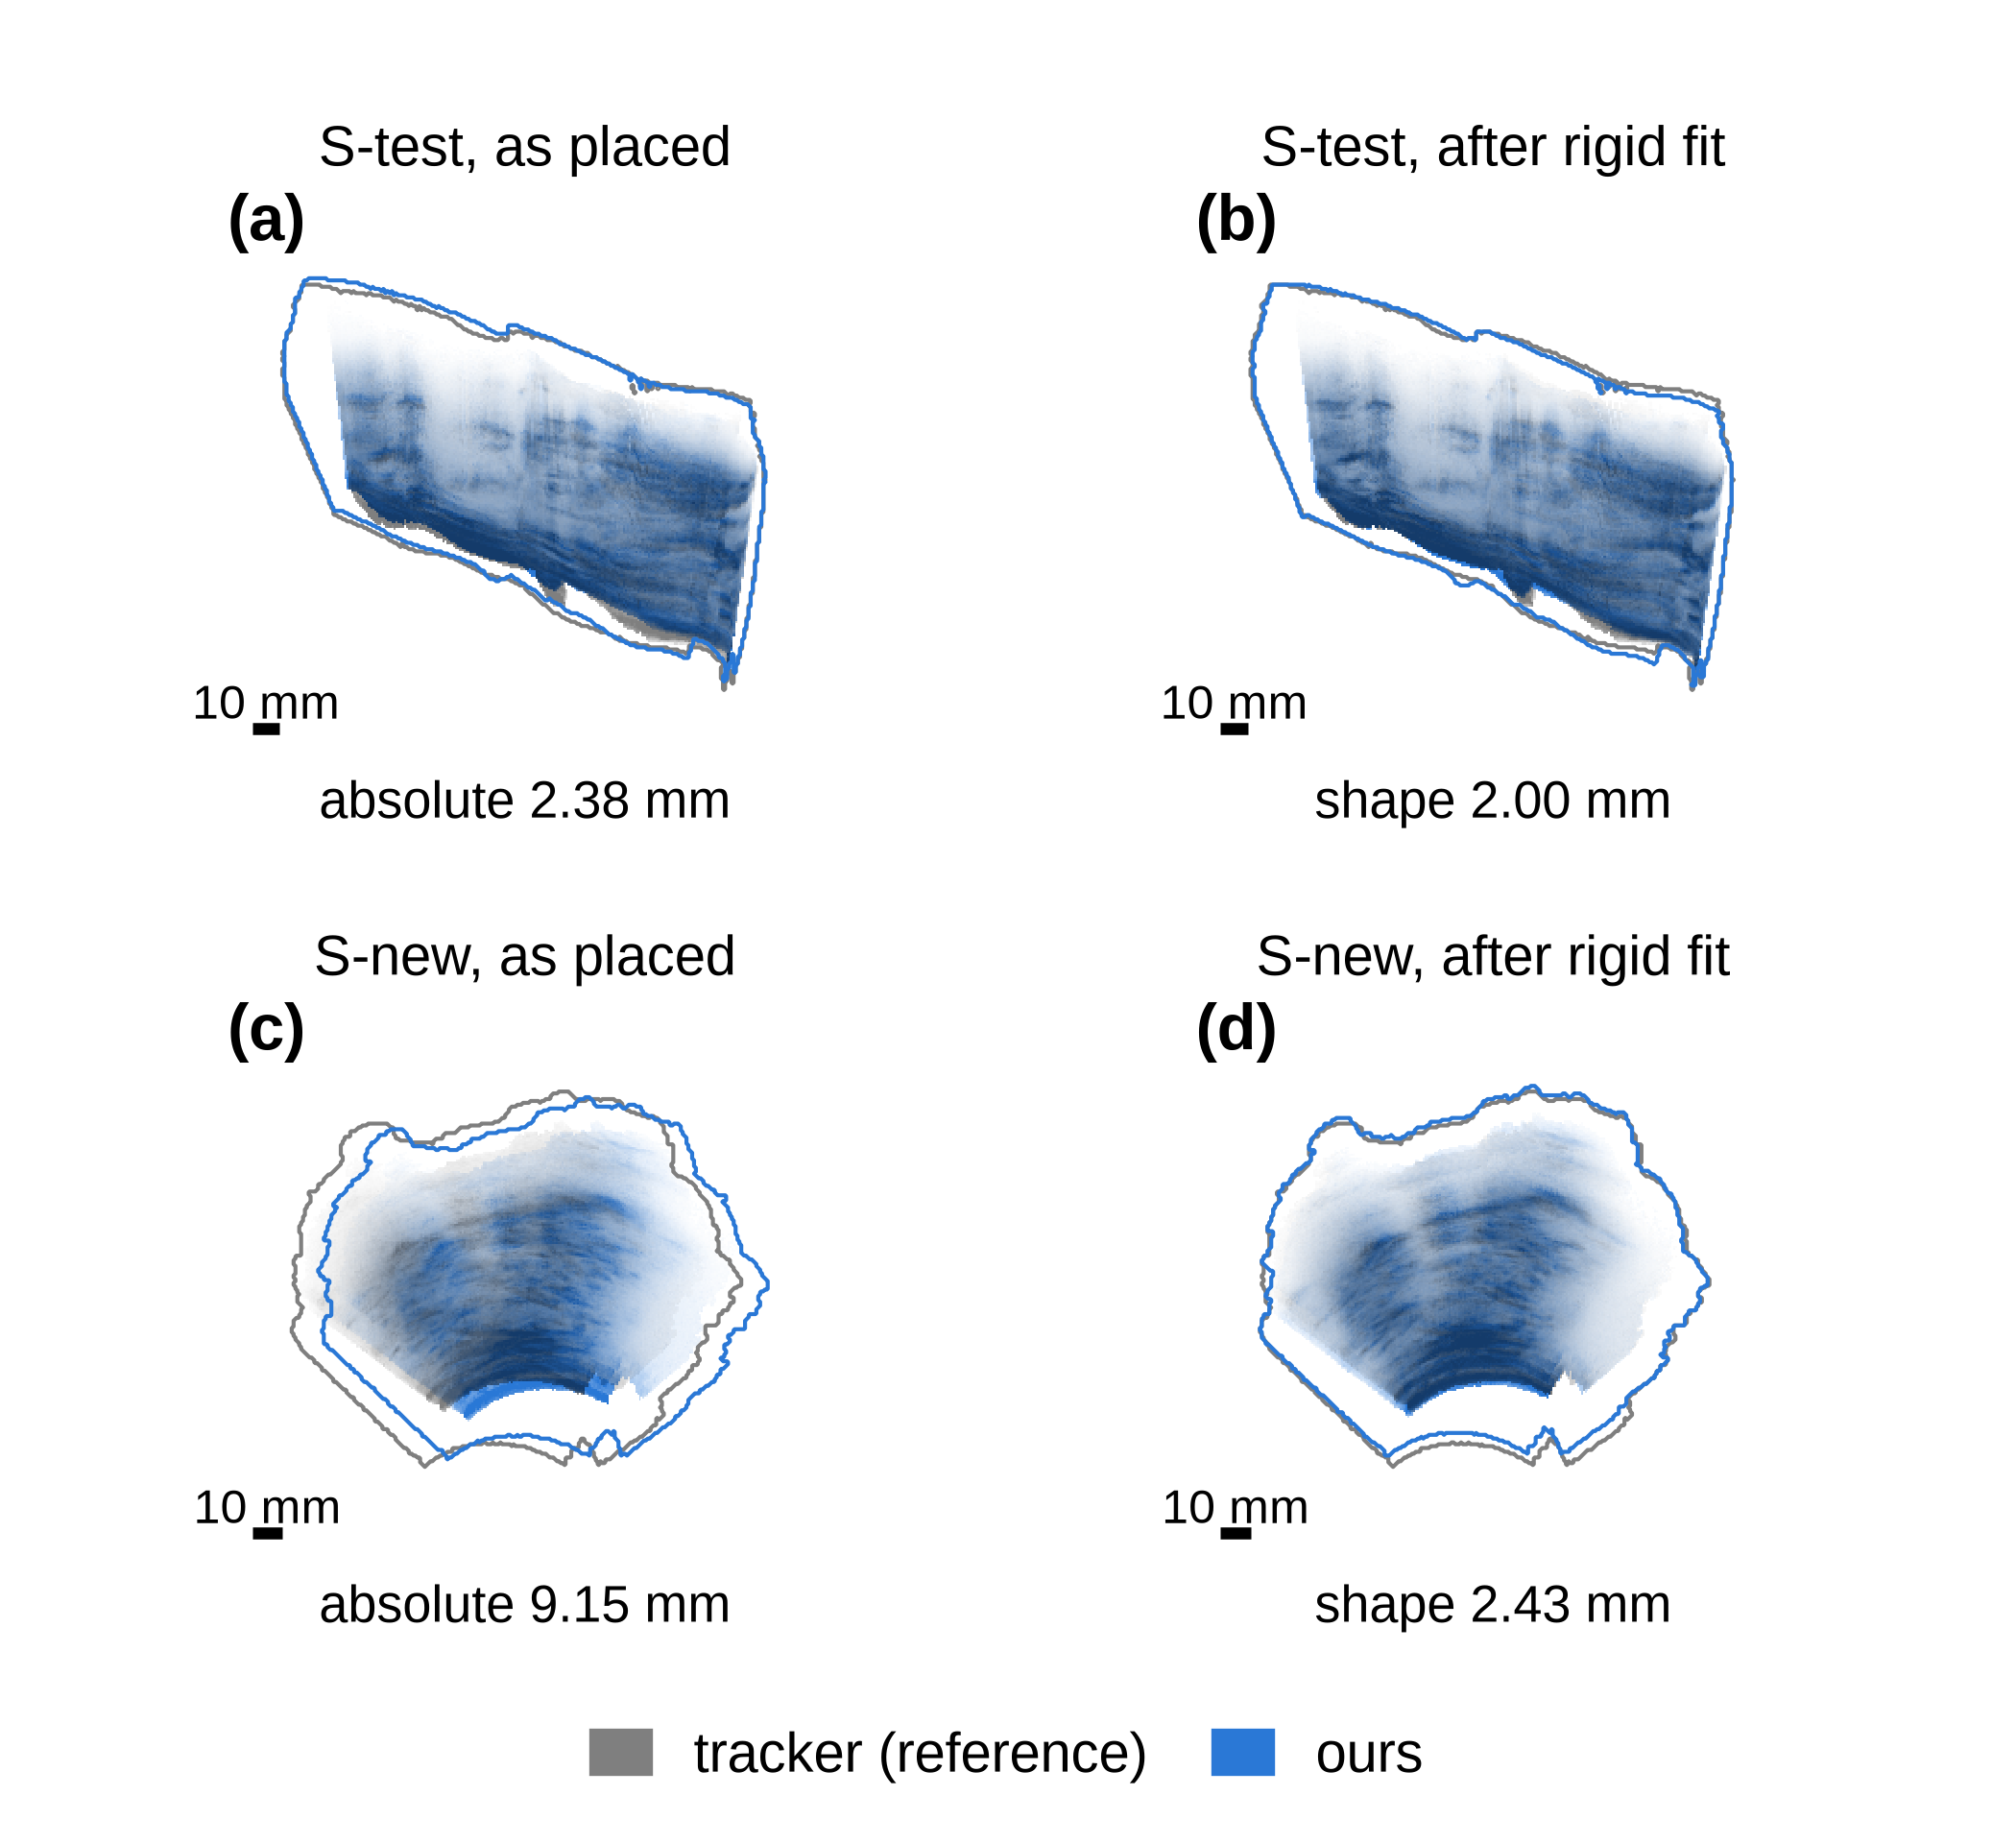
\includegraphics[width=0.90 \linewidth]{fig_volume_snew.png} 
  \caption{Tracker-free volumes as placed (left) and after the best rigid fit of the sweep (right), tracker poses in grey, ours in blue. (a,~b)~An \Stest{} sweep, with a room scan covering the sweeps: 2.38\,mm absolute, 2.00\,mm shape. (c,~d)~An \Snew{} sweep, with a short generic scan: 9.15\,mm absolute, 2.43\,mm shape. Without coverage the volume is displaced but keeps its shape. The two rows use different viewing directions (side view; B-mode plane), chosen so that the displacement lies in the image.}
  \label{fig:volume_snew}
\end{figure}

\emph{Scene changes.} People moving in the background (D, 2.24\,mm) and scanning after instead of before the sweeps (A, 2.50\,mm) did not raise the error. With an earlier block's map (Table~\ref{tab:ctrl}, lower part; 84--96\,\% of the views covered), A's map on B gives 4.28 / 3.00\,mm, similar to B's own scans. A's map on C gives 59.4\,mm with 21\,\% of frames posed, B's map on C 40.9\,mm with 96\,\% posed, and C's map on E 13.9\,mm (90th percentile 46.6\,mm); rescanning restores 3.11\,mm on C. The 400-inlier gate does not catch these failures; the median inlier count is 1371--2213 for current maps, 1126 for A's map on B and 23--450 for the failing cases (Fig.~\ref{fig:volume_outdated}). ORB-SLAM3 with B's map frozen did not track the first four C sweeps and is 19.2\,mm off on the other four; in full SLAM it is 43.7\,mm off as tracked and 4.65\,mm in the trajectory refined at shutdown. With C's map on E it gives 4.19\,mm.

\begin{figure}[t]
  \centering
  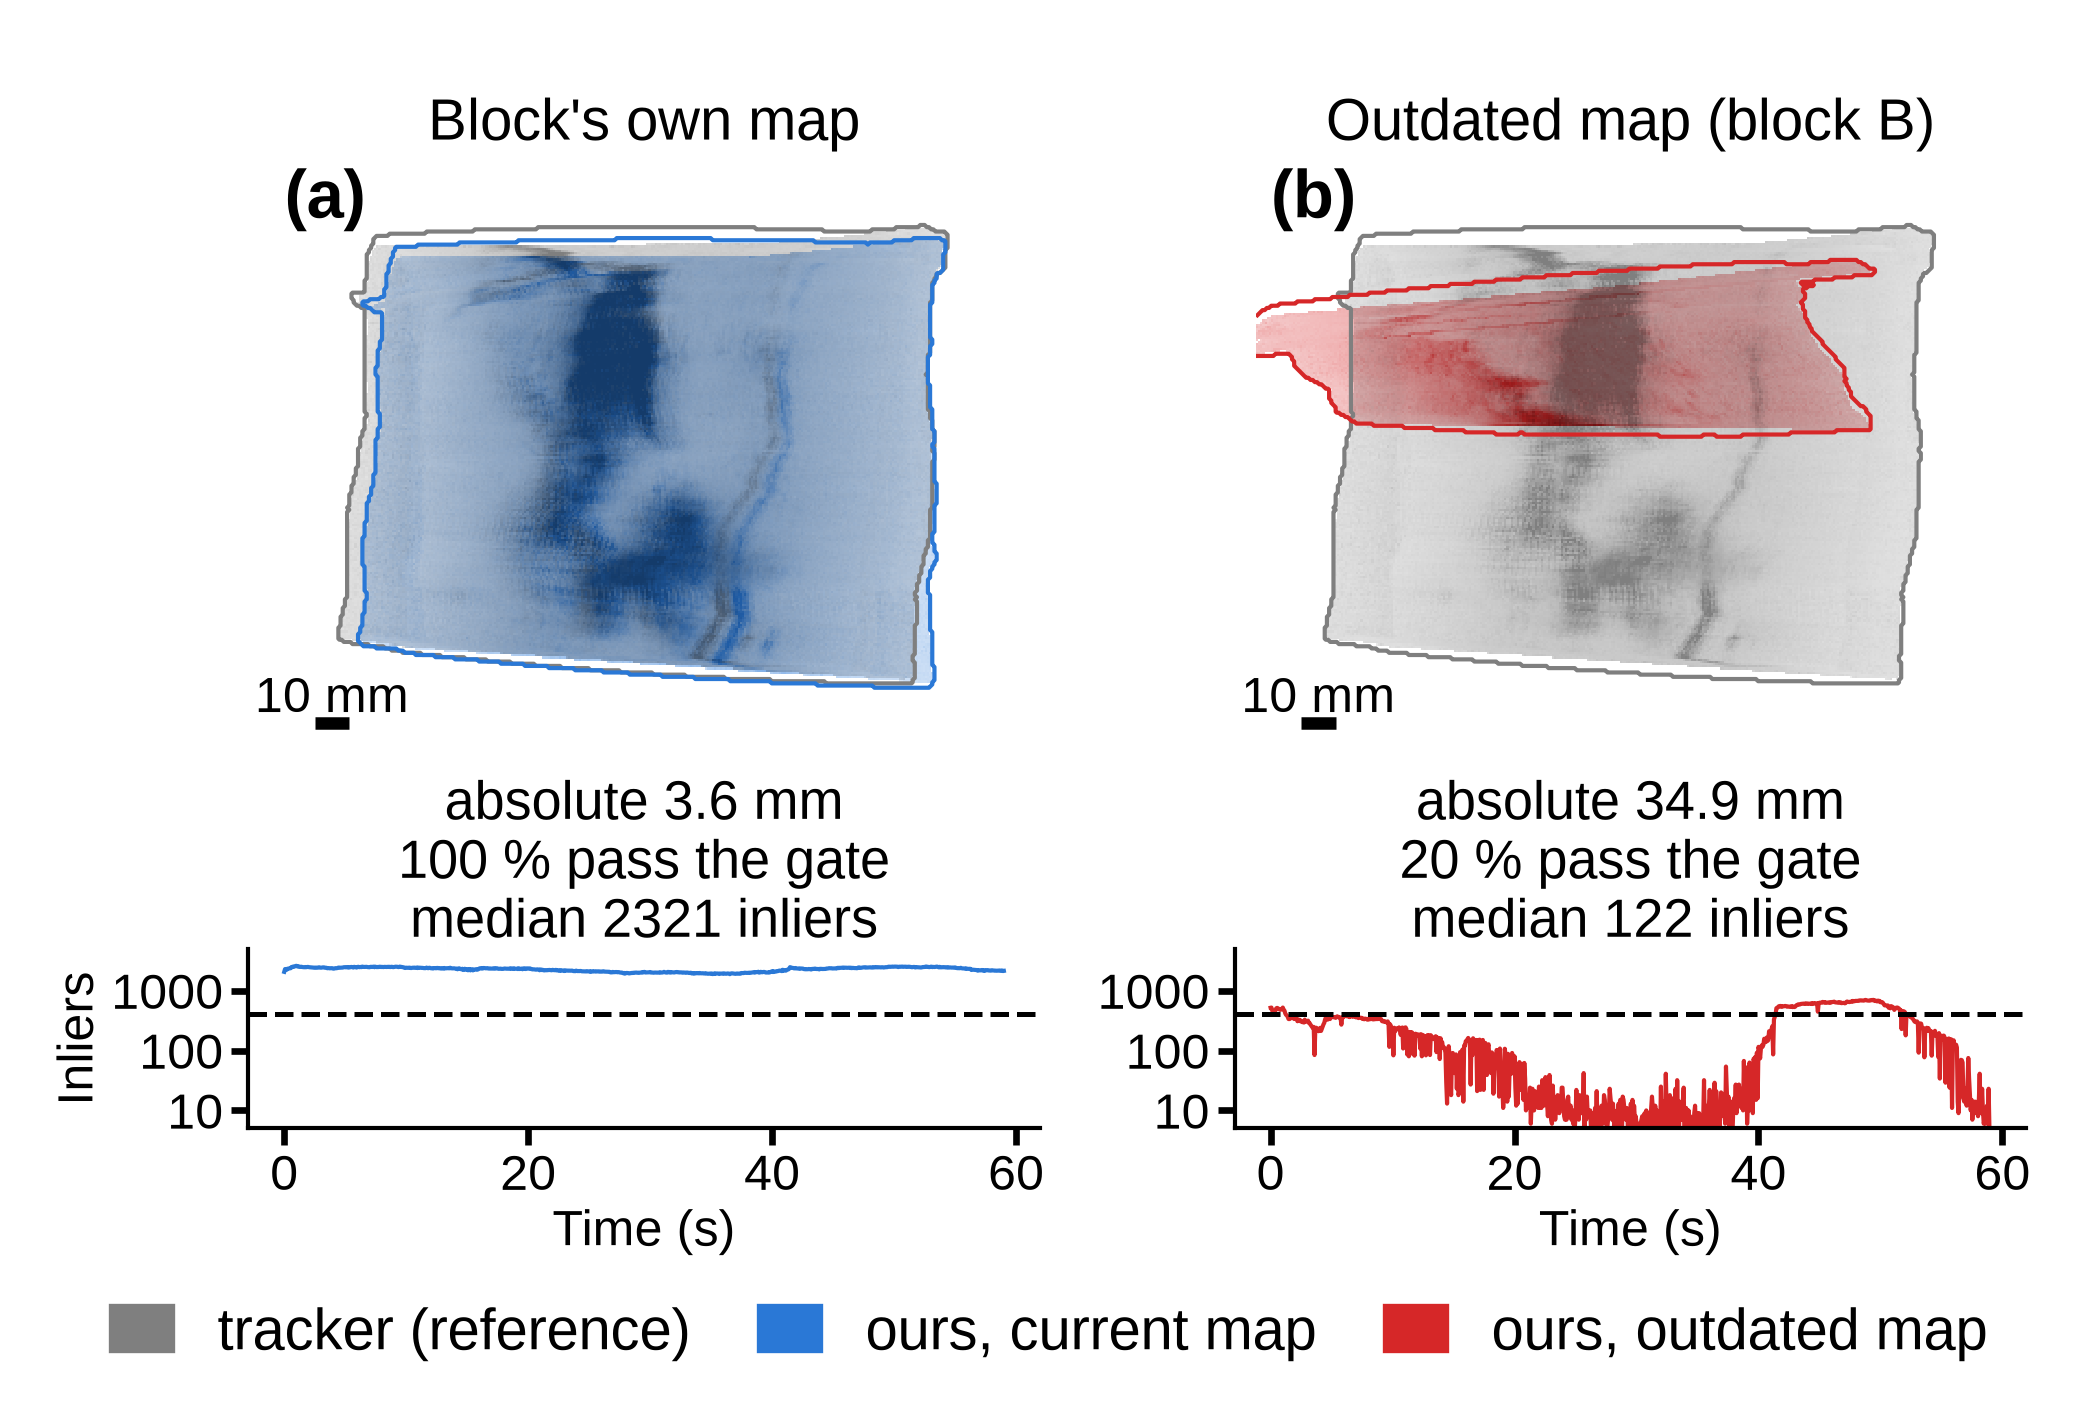
\includegraphics[width=0.90 \linewidth]{fig_volume_outdated.png} 
  \caption{An \Sctrl{} C sweep after a very large rearrangement, compounded with the block's own map (a) and with block B's outdated map (b); below, the Kabsch inlier count of every frame, with the 400-inlier gate dashed. Own map: 3.6\,mm, every frame passes the gate, median 2321 inliers. Outdated map: 34.9\,mm, 20\,\% of the frames pass, median 122 inliers. The median inlier count flags the outdated map without a tracker.}
  \label{fig:volume_outdated}
\end{figure}

\subsection{Comparison With Baselines and ORB-SLAM3}
\label{sec:res_compare}\label{sec:res_slam}
SCR anchors are about $8\times$ more accurate than pose-regression anchors (\Stest{} 1.8 vs.\ 15.3\,mm, \Snew{} 6.0 vs.\ 49.0\,mm). Against the classical pipeline, SCR is more accurate on \Stest{} (1.85 vs.\ 3.1\,mm with tracker-made maps; 2.35 vs.\ 3.65\,mm on our tracker-free map), equal under the strict protocol (2.98 vs.\ 3.0\,mm) and less accurate on \Snew{} (6.48 vs.\ 4.76\,mm); its shape error is lower on every split. The US-only method of Li et al.\ \cite{li2024longterm} reproduces its published accuracy on its own data (21.4 vs.\ 22.8\,mm) but is no better than assuming no motion on our sweeps, and fusing US with RGB does not improve on RGB alone (supplementary material).

ORB-SLAM3 is more accurate than our system in every session and mode (Table~\ref{tab:slam}, Fig.~\ref{fig:orbslam_persweep}). With each frame relocalised against its frozen map, it gives 1.72, 4.45 and 2.33\,mm on \Stest{}, \Snew{} and \Sctrl{}, against 2.34, 7.92 and 3.58\,mm for ours, and is lower on 52 of 63 sweeps (Wilcoxon $p<0.001$; mean paired difference \NUMQ{mean difference and 95\,\% bootstrap interval}). Its \Sctrl{} error changes little between modes (2.15\,mm in full SLAM as tracked, 2.36 in localisation only, 2.33 with each frame relocalised). With the generic \Sctrl{} A scan it gives 2.76\,mm, where ours gives 13.57\,mm. Ours is lower only on \Sctrl{} A with the exam-view scan (2.28 vs.\ 3.90\,mm, all 8 sweeps). Relocalising one frame takes ORB-SLAM3 25--41\,ms on the CPU (median) and our system 60--70\,ms on the GPU.

\begin{table*}[t]
  \caption{Comparison with ORB-SLAM3 (RGB-D) under the same protocol. Localisation only: map from the room scan, then frozen. Each frame relocalised: frozen map, every sweep frame relocalised with nothing from the previous frame. Session means of per-sweep medians at the US image, absolute / shape (mm); ORB-SLAM3 poses as tracked unless stated.}
  \label{tab:slam}
  \centering
  \scriptsize
  \setlength{\tabcolsep}{4pt}
  \begin{tabular}{@{}lccccc@{}}
    \toprule
    System & \Stest{} & \Snew{} & \Sctrl{} (exam-view) & \Sctrl{} A, generic scan & \Sctrl{} C, outdated scan\\
    \midrule
    Ours & 2.34 / 1.72 & 7.92 / 2.69 & 3.58 / 2.24 & 13.57 / 3.79 & 40.9 / 29.2\\
    ORB-SLAM3, full SLAM, refined at shutdown & 1.79 / 1.34 & 3.55 / 1.29 & 2.33 / 1.11 & -- & 4.65 / 1.15\\
    ORB-SLAM3, full SLAM & 1.81 / 1.18 & 4.47 / 2.28 & 2.15 / 1.08 & 3.16 / 1.09 & 43.69 / 3.51\\
    ORB-SLAM3, localisation only & 1.84 / 1.30 & 8.37 / 2.55 (A--D 4.45 / 1.34) & 2.36 / 1.27 & 2.88 / 1.19 & 19.19 / 10.58 (4 of 8 sweeps)\\
    ORB-SLAM3, each frame relocalised & 1.72 / 1.38 & 4.45 / 1.44 & 2.33 / 1.10 & 2.76 / 1.17 & 19.97 / 14.95 (3 of 8 sweeps)\\
    \bottomrule
  \end{tabular}
\end{table*}

\begin{figure}[t]
  \centering
  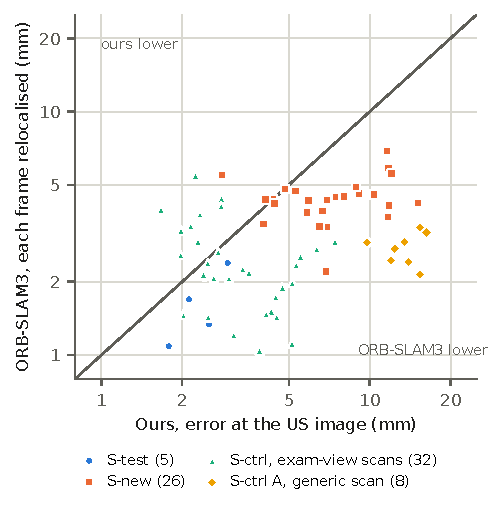
\includegraphics[width=0.90 \linewidth]{fig_orbslam_persweep.pdf} 
  \caption{Every test sweep, our error against ORB-SLAM3 with each frame relocalised against its frozen room-scan map (log scales). Points below the diagonal: ORB-SLAM3 lower (52 of 63 sweeps with current maps). Diamonds: \Sctrl{} A with the generic scan that misses the examination views.}
  \label{fig:orbslam_persweep}
\end{figure}


\subsection{Robustness to Occlusion}
\label{sec:res_occlusion}
With the synthetic occluder (Sec.~\ref{sec:occlusion}), our error rises by 0.4--0.9\,mm on average and no sweep exceeds 8.5\,mm; the inlier gate drops the frames that cannot be placed (87--100\,\% of frames posed) (Table~\ref{tab:occlusion}, Fig.~\ref{fig:occlusion}). ORB-SLAM3 stays more accurate on average, but in every mode it fails on single sweeps while reporting successful tracking for every frame: on \Sctrl{} B, 132\,mm in localisation only with 30\,\% occluded, and 38.6\,mm (full SLAM), 39.7\,mm (each frame relocalised) and 12.9\,mm (localisation only) with 60\,\% occluded. With 60\,\% occluded on \Sctrl{} C, it relocalises only 3 of 8 sweeps when each frame is relocalised. These failures also distort the volume: with 60\,\% occluded on \Sctrl{} B, the shape error is 3.88\,mm for ours and 7.35--8.44\,mm for ORB-SLAM3 in every mode. The same pattern appeared without a synthetic occluder in \Snew{} E, where an arm crossed the view in two sweeps: localisation-only ORB-SLAM3 was 81.5\,mm off on one of them in one run and 28.2\,mm in another, while ours gave 6.9\,mm. The failures are rare and vary from run to run; the evidence covers two blocks and one occluder.

\begin{table*}[t]
  \caption{Controlled occlusion on \Sctrl{} B and C (8 sweeps each): mean of per-sweep medians at the US image, worst sweep in brackets, then shape (mm). Occluded: share of the image width covered by the occluder.}
  \label{tab:occlusion}
  \centering
  \scriptsize
  \setlength{\tabcolsep}{5pt}
  \begin{tabular}{@{}lcccc@{}}
    \toprule
    Block, occluded & Ours & ORB-SLAM3, full SLAM & localisation only & each frame relocalised\\
    \midrule
    B, none & 4.43 (6.3) / 2.81 & 1.79 / 1.22 & 1.70 / 1.17 & 1.63 / 1.20\\
    B, 30\,\% & 5.16 (7.5) / 3.38 & 1.76 (2.9) / 1.44 & 17.91 (132.2) / 6.14 & 1.78 (2.9) / 1.59\\
    B, 60\,\% & 5.28 (8.5) / 3.88 & 6.88 (38.6) / 7.42 & 3.32 (12.9) / 8.44 & 6.72 (39.7) / 7.35\\
    C, none & 3.11 (5.1) / 1.76 & 1.67 / 1.09 & 2.05 / 1.11 & 2.27 / 1.06\\
    C, 30\,\% & 3.54 (6.1) / 2.27 & 2.12 (2.6) / 1.15 & 2.48 (2.9) / 1.38 & 2.01 (2.3) / 1.32\\
    C, 60\,\% & 3.89 (6.6) / 2.80 & 2.67 (3.3) / 1.83 & 2.65 (3.1) / 2.29 & 2.22 (2.5) / 3.20, 3 of 8 sweeps\\
    \bottomrule
  \end{tabular}
\end{table*}

\begin{figure}[t]
  \centering
  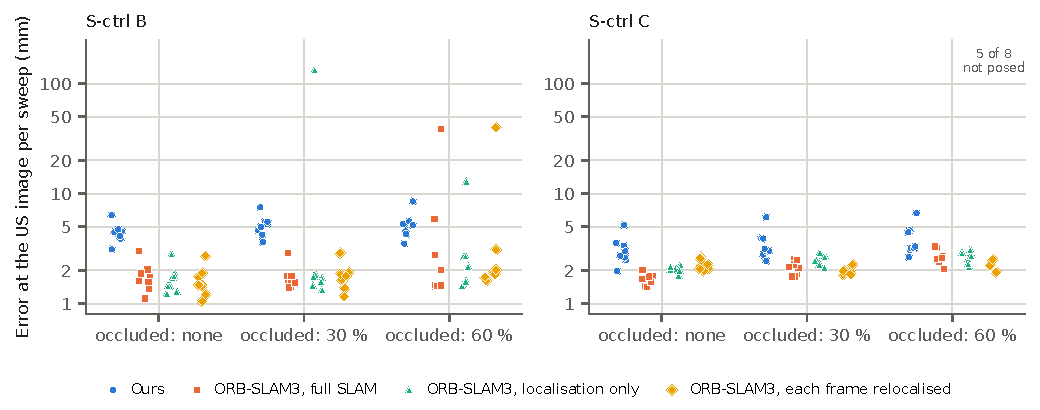
\includegraphics[width=0.90 \linewidth]{fig_occlusion.pdf} 
  \caption{Controlled occlusion on \Sctrl{} B and C: per-sweep error at the US image without the occluder and with 30\,\% or 60\,\% of the image width occluded (log scale). Each point is one sweep. Our error stays bounded; ORB-SLAM3 is lower on average but fails on single sweeps while reporting successful tracking.}
  \label{fig:occlusion}
\end{figure}


\subsection{Robustness to Occlusion}
\label{sec:res_occlusion}
With the synthetic occluder (Table~\ref{tab:occlusion}, Fig.~\ref{fig:occlusion}), our mean error rises by 0.4--0.9\,mm, no sweep exceeds 8.5\,mm, and 87--100\,\% of the frames are posed. ORB-SLAM3 has the lower mean error in 9 of the 12 occluded settings, but in every mode single sweeps fail while every frame is reported as tracked: on \Sctrl{} B, 132\,mm in localisation only with 30\,\% occluded, and 38.6\,mm (full SLAM), 39.7\,mm (each frame relocalised) and 12.9\,mm (localisation only) with 60\,\% occluded. With 60\,\% occluded on \Sctrl{} C, it relocalises 3 of 8 sweeps when each frame is relocalised. With 60\,\% occluded on \Sctrl{} B, the shape error is 3.88\,mm for ours and 7.35--8.44\,mm for ORB-SLAM3. On \Snew{} E, where an arm crossed the view in two sweeps without a synthetic occluder, localisation-only ORB-SLAM3 was 81.5\,mm off on one of them in one run and 28.2\,mm in another, and ours 6.9\,mm.

\begin{table*}[t]
  \caption{Controlled occlusion on \Sctrl{} B and C (8 sweeps each): mean of per-sweep medians at the US image, worst sweep in brackets, then shape (mm). Occluded: share of the image width covered by the occluder.}
  \label{tab:occlusion}
  \centering
  \scriptsize
  \setlength{\tabcolsep}{5pt}
  \begin{tabular}{@{}lcccc@{}}
    \toprule
    Block, occluded & Ours & ORB-SLAM3, full SLAM & localisation only & each frame relocalised\\
    \midrule
    B, none & 4.43 (6.3) / 2.81 & 1.79 / 1.22 & 1.70 / 1.17 & 1.63 / 1.20\\
    B, 30\,\% & 5.16 (7.5) / 3.38 & 1.76 (2.9) / 1.44 & 17.91 (132.2) / 6.14 & 1.78 (2.9) / 1.59\\
    B, 60\,\% & 5.28 (8.5) / 3.88 & 6.88 (38.6) / 7.42 & 3.32 (12.9) / 8.44 & 6.72 (39.7) / 7.35\\
    C, none & 3.11 (5.1) / 1.76 & 1.67 / 1.09 & 2.05 / 1.11 & 2.27 / 1.06\\
    C, 30\,\% & 3.54 (6.1) / 2.27 & 2.12 (2.6) / 1.15 & 2.48 (2.9) / 1.38 & 2.01 (2.3) / 1.32\\
    C, 60\,\% & 3.89 (6.6) / 2.80 & 2.67 (3.3) / 1.83 & 2.65 (3.1) / 2.29 & 2.22 (2.5) / 3.20, 3 of 8 sweeps\\
    \bottomrule
  \end{tabular}
\end{table*}

\begin{figure}[t]
  \centering
  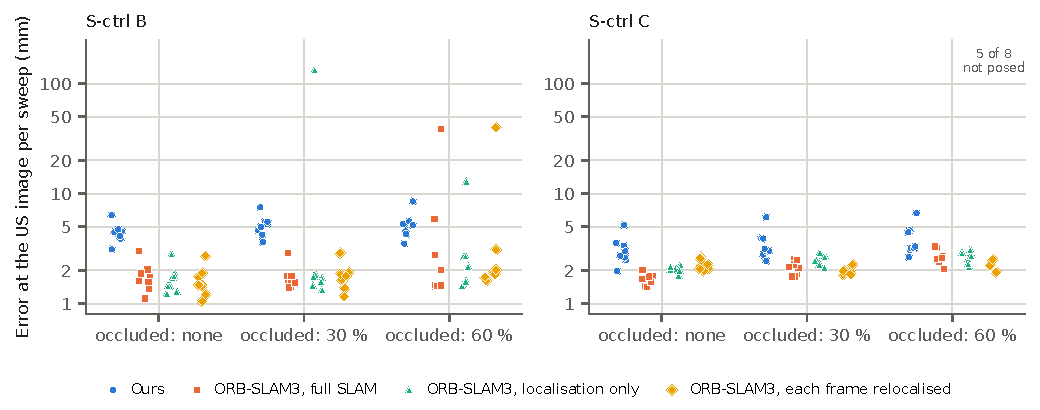
\includegraphics[width=0.90 \linewidth]{fig_occlusion.pdf} 
  \caption{Controlled occlusion on \Sctrl{} B and C: per-sweep error at the US image without the occluder and with 30\,\% or 60\,\% of the image width occluded (log scale). Each point is one sweep. Our error stays bounded; ORB-SLAM3 is lower in most settings but fails on single sweeps while reporting successful tracking.}
  \label{fig:occlusion}
\end{figure}





%======================================================================
\section{Discussion}
\label{sec:discussion}
%======================================================================

With a room scan along the examination views, the system reaches 2.2--3.1\,mm at the US image and 1.7--1.9\,mm volume shape error in two sessions, with nothing outside the probe during the examination. Removing the tracker from mapping costs 0.4--0.5\,mm relative to the same network on tracker labels.

A network that learns the room from a scan is accurate only near the viewpoints of that scan: with perfect labels, a scan that misses the examination views still gives 10.95\,mm instead of 1.85\,mm. This is a limit of regressing scene coordinates, not of self-mapping and not of mapping the room before the examination: ORB-SLAM3 with the same generic scan, frozen, gives 2.76\,mm, because its keypoints can be matched from new viewpoints. For the operator, the consequence is concrete: scan along the planned sweep paths, which takes about 1--2\,min. More footage does not substitute for the right footage: adding a generic scan made the map worse (3.15 vs.\ 2.28\,mm). Training that makes scene coordinate networks extrapolate to new viewpoints, as ACE-G does for RGB \cite{bruns2025aceg}, is the most direct way to relax this requirement.

Between nearby frames all systems agree (out-of-plane error over 8 rows 0.23--0.37\,mm on \Stest{}). The tracker-free error is mostly a placement of the whole sweep in the room rather than a distortion of it: with poor coverage our shape error stays the lowest of our system, the oracle map and the classical pipeline in \Snew{} while the absolute error is the largest. For volume measurements that need no registration to other images, shape is the relevant error; for navigation in a room frame, the absolute error is.

Pose regression and SCR are both learned and both see the room scan, yet their anchor errors differ by about $8\times$. A pose-regression network merges the whole image into one pose, which moved objects or hands corrupt; SCR predicts 3600 independent correspondences, RANSAC keeps the consistent ones, and a rigid fit through thousands of them averages the noise. SCR is retrained per room, so memorising the room is its task, and the same property lets it map its own scan. Depth helps twice: for metric labels, and for a 3D--3D solve that is more accurate than PnP. End-to-end fine-tuning through the differentiable Kabsch fit, as in DSAC* \cite{brachmann2022dsac}, was not needed, because the map rather than the solver limits the accuracy; and $X$ cannot be learned from the images, because it relates the camera frame to the tracker's hand--eye frame.

Once coverage is sufficient, the error follows the map's camera error plus about 1\,mm. An emptied room gives poor maps, because depth ICP has little structure to align. Better maps could come from a joint refinement with depth constraints, or from adding a few known objects to an empty room.

RGB-D SLAM is the established way to track a probe camera against the room \cite{busam2018insideout}, and ORB-SLAM3 is more accurate than our system in every session, also when both use only the room scan; we do not claim higher accuracy. The comparison shows where the difference lies. It is not the tracking over time and not mapping during the examination: ORB-SLAM3 keeps its accuracy with its map frozen and every frame relocalised on its own. It is the map: sparse keypoints with descriptors generalise to viewpoints the room scan missed, and a network that regresses room coordinates does not. What the learned, per-frame approach offers instead is a different failure behaviour. It holds no tracking state, so a wrong pose is not carried into the next frame, and its error stays bounded when part of the view is blocked (no sweep above 8.5\,mm with 60\,\% of the image occluded). ORB-SLAM3, more accurate on average, occasionally loses a whole sweep by tens of millimetres while reporting successful tracking, in every mode, and these failures vary from run to run. For compounding, a silent failure of a whole sweep is harder to handle than a known, bounded error. The two approaches are complementary: ORB-SLAM3 could be guarded by an independent per-frame check, and per-frame scene coordinate relocalisation could be used inside SLAM, as in ACE-SLAM \cite{alzugaray2025aceslam}.

Low coverage is silent: every frame passes the inlier gate, and only the coverage check catches it. An outdated map after a very large change fails with low inlier counts, which a session-level median-inlier check flags; ORB-SLAM3 fails in the same situation when run live. An empty room gives a poor map, which the map error reveals only with a reference; this case calls for adding structure to the room. Occlusion of part of the view degrades our error gradually rather than abruptly.

Preparation per room takes about 30\,min of self-mapping and 13--40\,min of training, and tracking runs at 60--70\,ms per frame. The probe calibration $X$ is needed once per probe and would come from a phantom; across sessions, its transfer adds part of the placement error (\Snew{} C 9.40 vs.\ 7.87\,mm after refitting), so a periodic recalibration may be needed.


ORB-SLAM3 is more accurate than our system in every session, also like for like, and does not need the room scan to cover the examination views. Its localisation mode needed a one-line change to relocalise after tracking failures, and it varies from run to run, so single runs of it should be read with care. The occlusion experiment uses one synthetic occluder on two blocks; real hands and arms differ in shape, motion and depth. All data come from one room, two subjects and one phantom, and the test sets are small (5 + 26 + 32 sweeps). $X$ was fitted with the tracker, and the coverage check was computed with the tracker, so the workflow is not yet fully tracker-free. The ground truth was recorded at the near edge of the tracker volume; no trend with distance was found, but a common bias cannot be excluded, and the hand--eye error enters the ground truth. The median-inlier threshold was not tuned on independent data. The tracking ablations and the frame-level coverage analysis use the oracle map; their transfer to a self-made map is assumed. The pooled-scan variant was examined on \Snew{} test blocks. Real time was shown on recorded data, not live.

%======================================================================
\section{Conclusion}
%======================================================================
A probe-mounted RGB-D camera and one scene coordinate network that maps its own room scan give the pose of every freehand US frame without an external tracker. With a room scan along the examination views, the error at the US image is 2.2--3.1\,mm in two sessions, 0.4--0.5\,mm more than with tracker labels. Coverage of the examination views decides the accuracy, then map quality, then scene changes; a short exam-view scan, a coverage check and an inlier check make these conditions explicit before the examination. ORB-SLAM3 is more accurate and does not need this coverage; the learned per-frame approach offers a bounded error under occlusion and detectable failures instead. Scene coordinate networks that generalise to new viewpoints, and their combination with SLAM, are the directions that would close the gap.


\section*{Acknowledgment}



\bibliographystyle{IEEEtran}
\bibliography{bib}


\end{document}